
\documentclass[letterpaper,11pt]{article}

\usepackage[letterpaper, margin=0.75in]{geometry}
\usepackage{titlesec}
\usepackage[document]{ragged2e}
\usepackage{gensymb}
\usepackage{textcomp}
\usepackage{graphicx}
\usepackage{subfig}
\usepackage{float}
\usepackage{wrapfig}
\usepackage{setspace}

\setlength{\parskip}{1em}

\DeclareGraphicsExtensions{.jpg,.JPG}

\newcommand*{\TitleFont}{
      \usefont{\encodingdefault}{\rmdefault}{b}{n}
      \fontsize{12}{5}
      \selectfont}

\newcommand\blankpage{%
    \null
    \thispagestyle{empty}%
    %\addtocounter{page}{-1}%
    \newpage}
      
\begin{document}
\begin{center}
\TitleFont AIT Measurement Standard Operating Procedure\newline
\TitleFont Last modified on: \today \hspace{1mm} by Mark Redd \newline
\end{center}

\titleformat{\section}
  {\normalfont\fontsize{12}{15}\bfseries}{\thesection}{1em}{}

\begin{itemize}
\item \textbf{NOTICE: Lab policy requires that any person performing 
    AIT measurements must have done the following before performing any 
    experimental work:}
    
    \begin{itemize}
    \item \textbf{Complete pertinent laboratory safety training 
    \item Read this SOP in its entirety
    \item Become familiar with all the experimental steps outlined in this SOP
    \item Sign and Date the AIT SOP Signatures Sheet}
    \end {itemize}
\end{itemize}
\renewcommand{\baselinestretch}{.4}\normalsize
\tableofcontents    % insert the table of contents
\renewcommand{\baselinestretch}{1.0}\normalsize

        

\newpage

\section{Measurement and Data Collection}
This section enumerates the procedure for measuring AIT. Researchers 
should follow these procedures every day and for every experiment performed to 
ensure consistent results. The first priority should always be safety. 
Therefore, if any step of this process is found to be unsafe or pose an 
unacceptable risk it should be changed. Furthermore, changes should be made if 
any step of the process violates the ASTM E659 Method to conform to the 
requirements of the method.
    
    \subsection{Startup}
    
    \begin{enumerate}
    \item Ensure the lid is off the pressure vessel and the vessel is being 
        vented by the snorkel
        \begin{itemize}
        \item Under normal operation, the vessel should be vented with the 
            snorkel any time the vessel is open
        \item The only exception to this rule is when the experimental setup has
            been shut down for an extended period of time for maintenance 
            purposes
        \end{itemize}
    
    \item Ensure the furnace is plugged in to the 220 V outlet on the edge of 
        the hood
    \item Power on the furnace and set furnace temperature between 10 - 20 
        degrees above your initial target flask temperature 
        \begin{itemize}
        \item When powered on initially, the furnace may take 2 hours or   
            more to reach a desired temperature and thermally equilibrate
        \item Use the TADA\_UI to track the internal temperature of the flask
        \item Once the internal temperature starts to reach equilibrium, you 
            may adjust the set point temperature until the target 
            temperature is reached
        \item \textbf{CAUTION: The furnace may be hot during the start up 
            sequence. Avoid touching anything inside the area enclosed by 
            the aluminum ring atop the furnace including the ring itself.}
        \end{itemize}
    
    \item Ensure the vessel rupture disk is intact and positioned correctly 
        (See Figure \ref{fig:rupture_disk})
        \begin{itemize}
        \item See the training on proper rupture disk installation if the this is not the case
        \end{itemize} 
    
\begin{figure}[H]
\centering
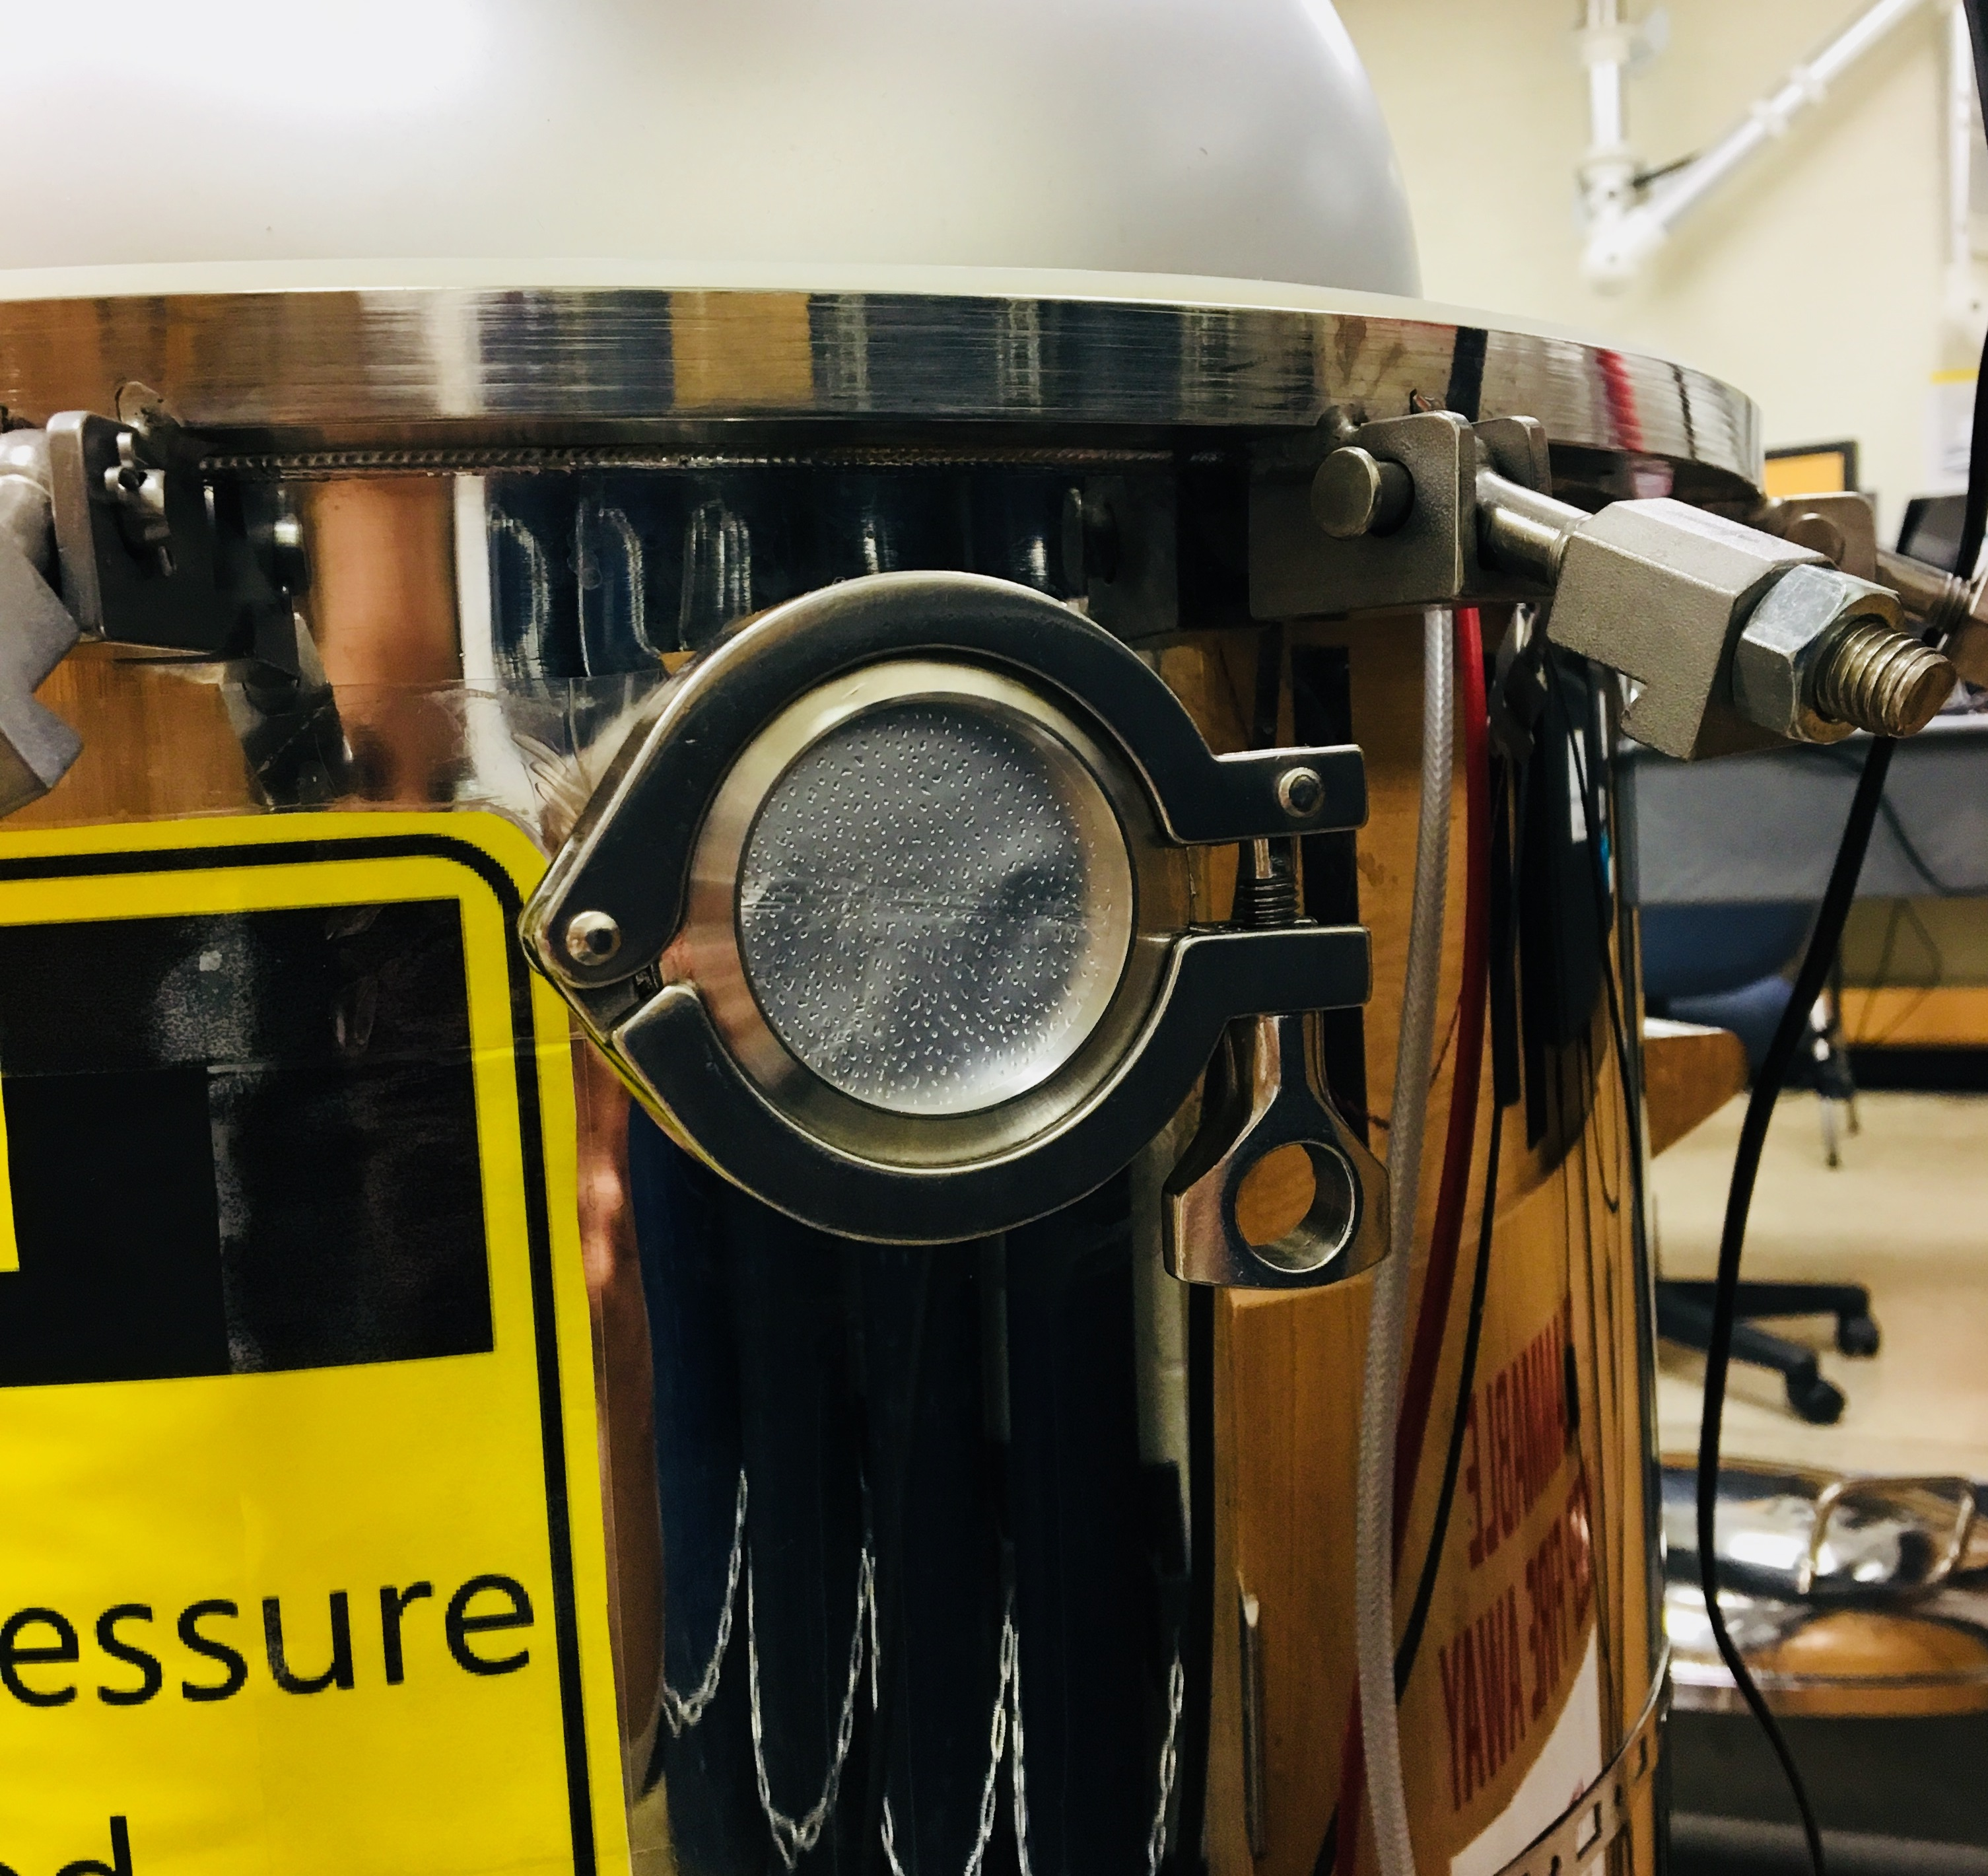
\includegraphics[width=.25\textwidth]{rupture_disk.jpg}
\caption{Ensure the rupture disk is present and intact}
\label{fig:rupture_disk}
\end{figure}
    
    \item Start up computer and log on
        \begin{itemize}
      
        \item Use your CAEDM account to log in
            \begin{itemize}
            \item You should be able to access all the needed tools and 
                programs from your account
            \item If you cannot access a program or file from your account, let 
                Mark know and he will give you administrator access as needed
            \end{itemize}
        
        \item You may need to specify the domain you are logging into. If that 
            is the case enter your CAEDM credentials in as follows:
            \begin{itemize}
            \item Username: CAEDM\_AD\textbackslash
            \textit{your\_caedm\_username}
            \item Password: \textit{your\_caedm\_password}
            \end{itemize}
        
        %\item Using the administrator account:
        %    \begin{itemize}
        %    \item Username: CHEME-R-2014-25\textbackslash AIT\_LAB
        %    \item Password: Explosionsinthesky16 (Explosions in the sky 16)
        %    \end{itemize}
        %    Username: cheme-r-2014-25\AIT_LAB
        %    Password: Explosionsinthesky16 (Explosions in the sky 16)
        
        \end{itemize}
    
    \item Ensure a compatible SD card is inserted securely into the TADA 
        datalogger (see Figure \ref{fig:sd_card_reader})
        
\begin{figure}[H]
\centering
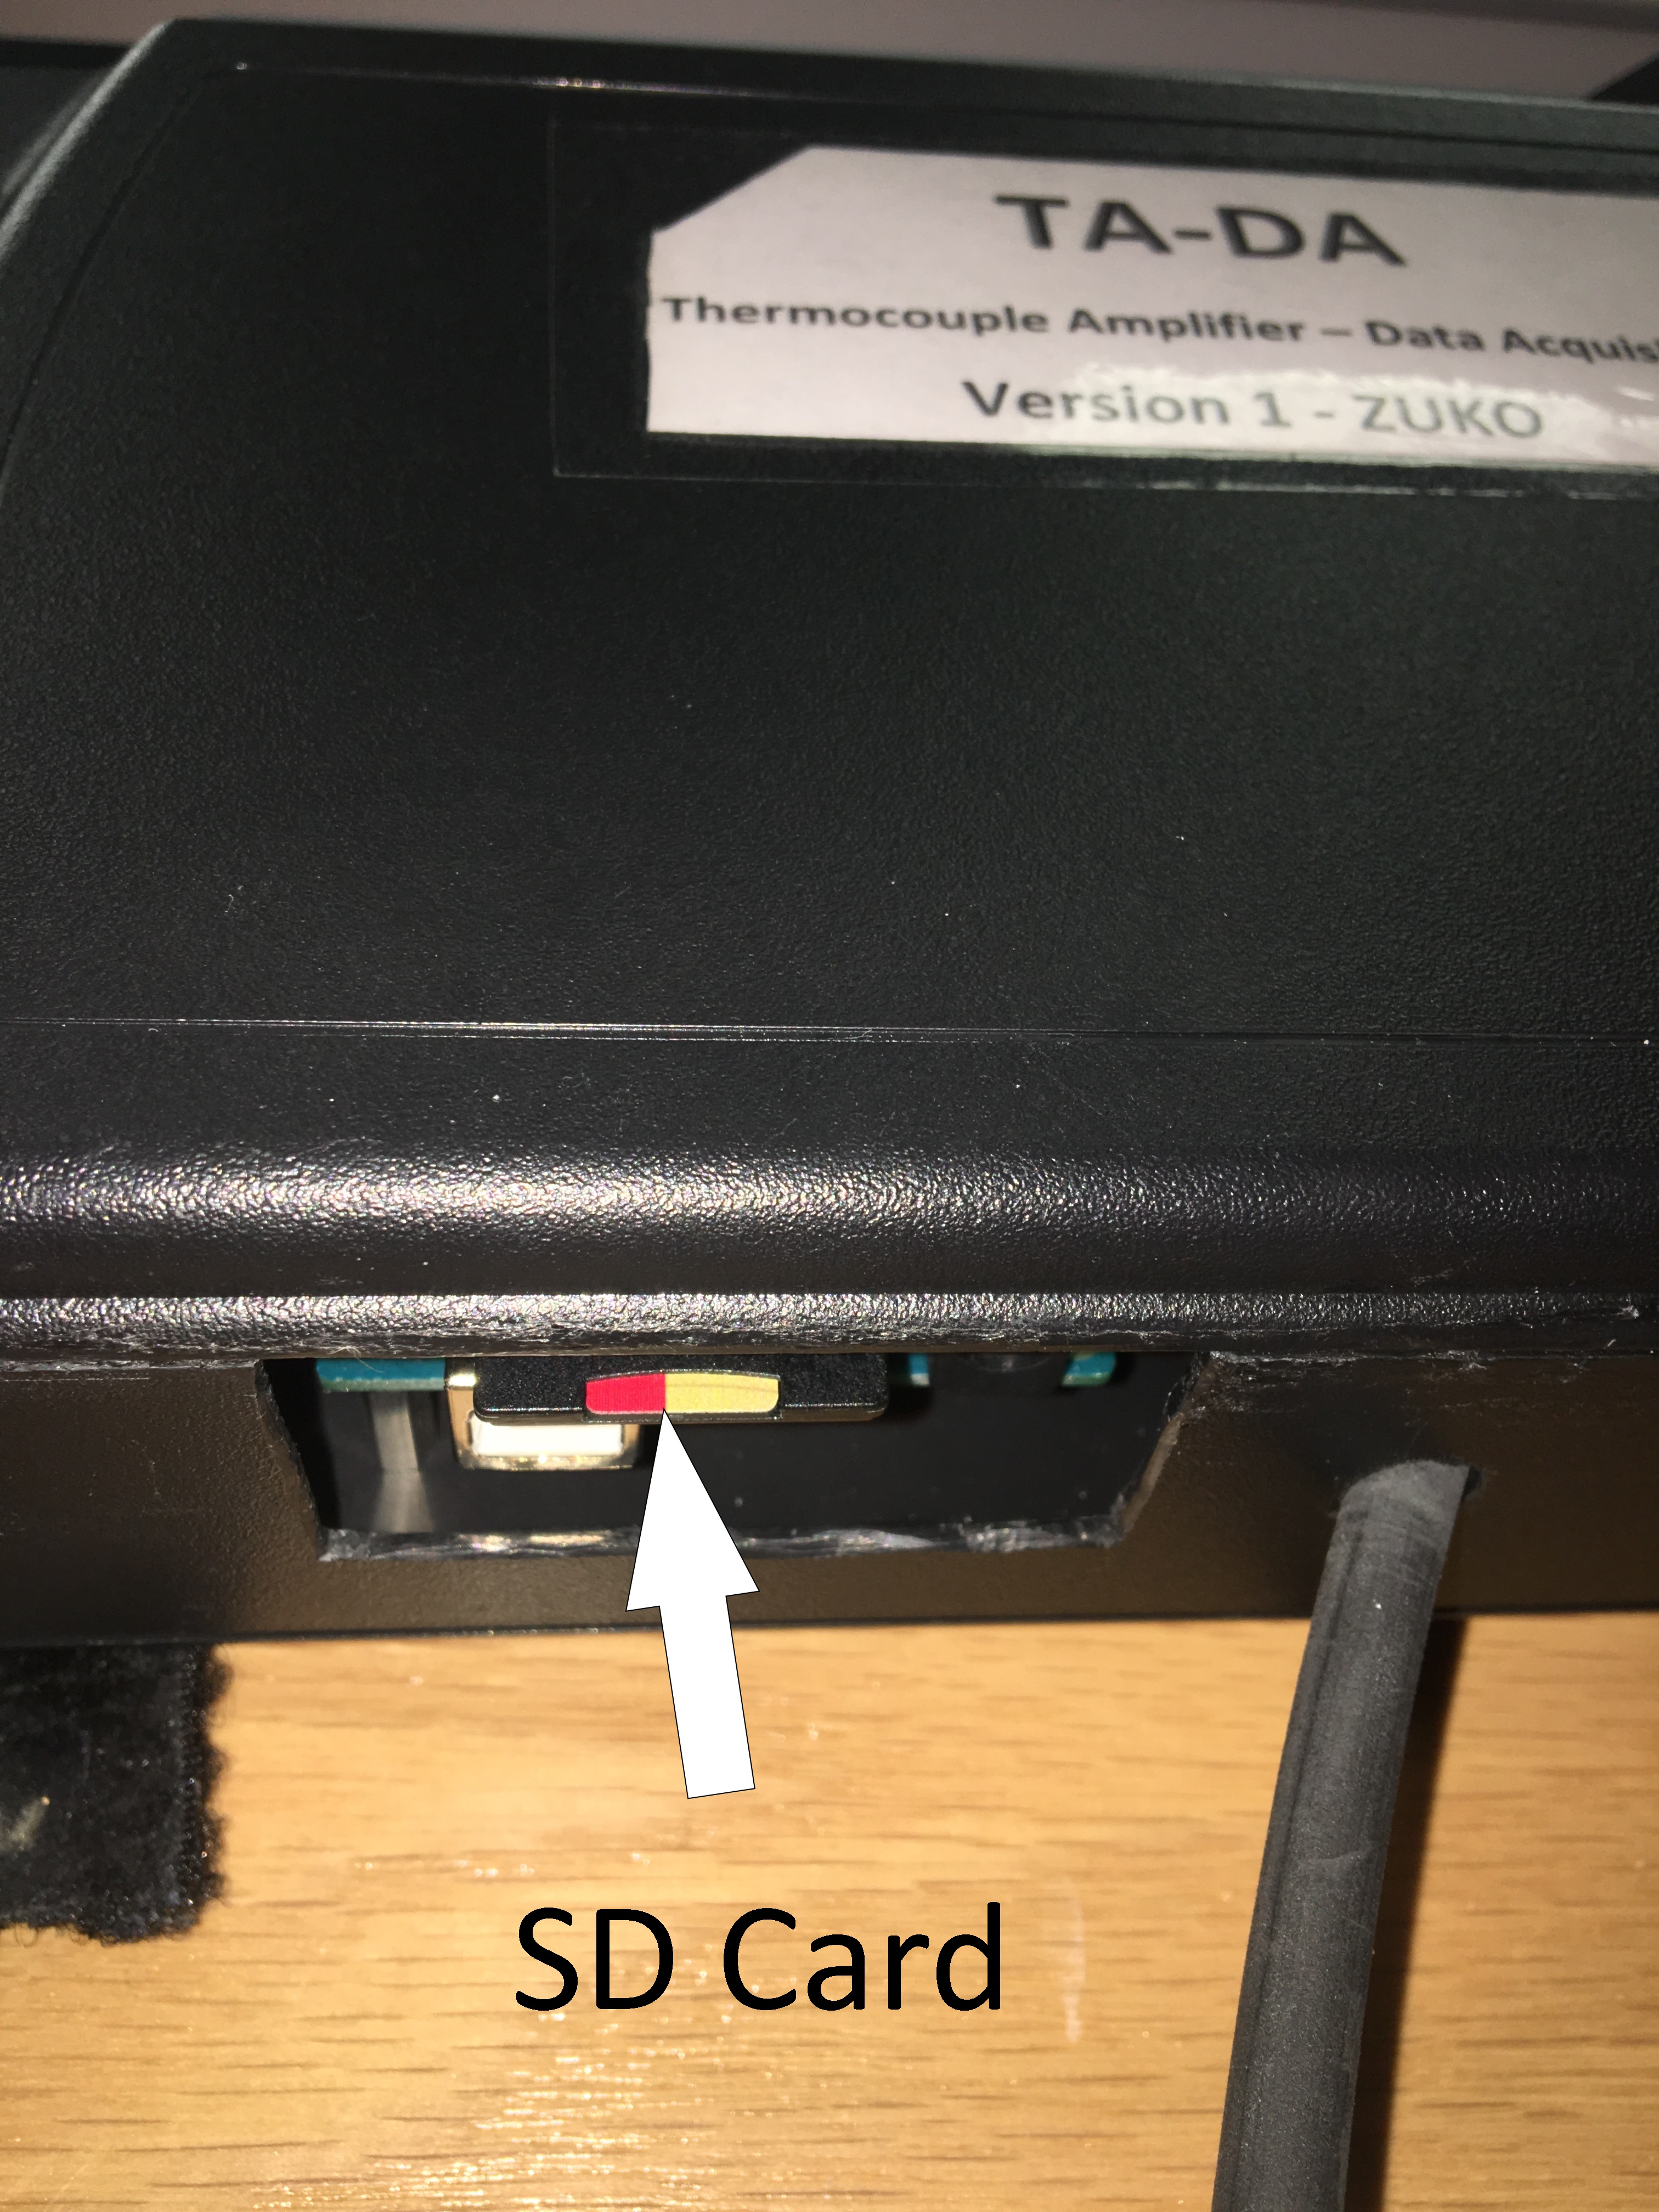
\includegraphics[width=.3\textwidth]{sd_card_reader.jpg}
\caption{SD card slot location}
\label{fig:sd_card_reader}
\end{figure}
        
    \item Ensure the 4 furnace thermocouples are connected to their 
        corresponding connectors inside the vessel and ensure that the wires are
        tucked down between the side of the furnace and the wall of the vessel 
        and are out of the way (see Figure \ref{fig:Thermocouples})
        \begin {itemize}
        \item Thermocouple wires coming out of the furnace are numbered and
            should connect to the corresponding brown wire connected to 
            the TA-DA
        \end{itemize}
        
\begin{figure}[H]
\centering
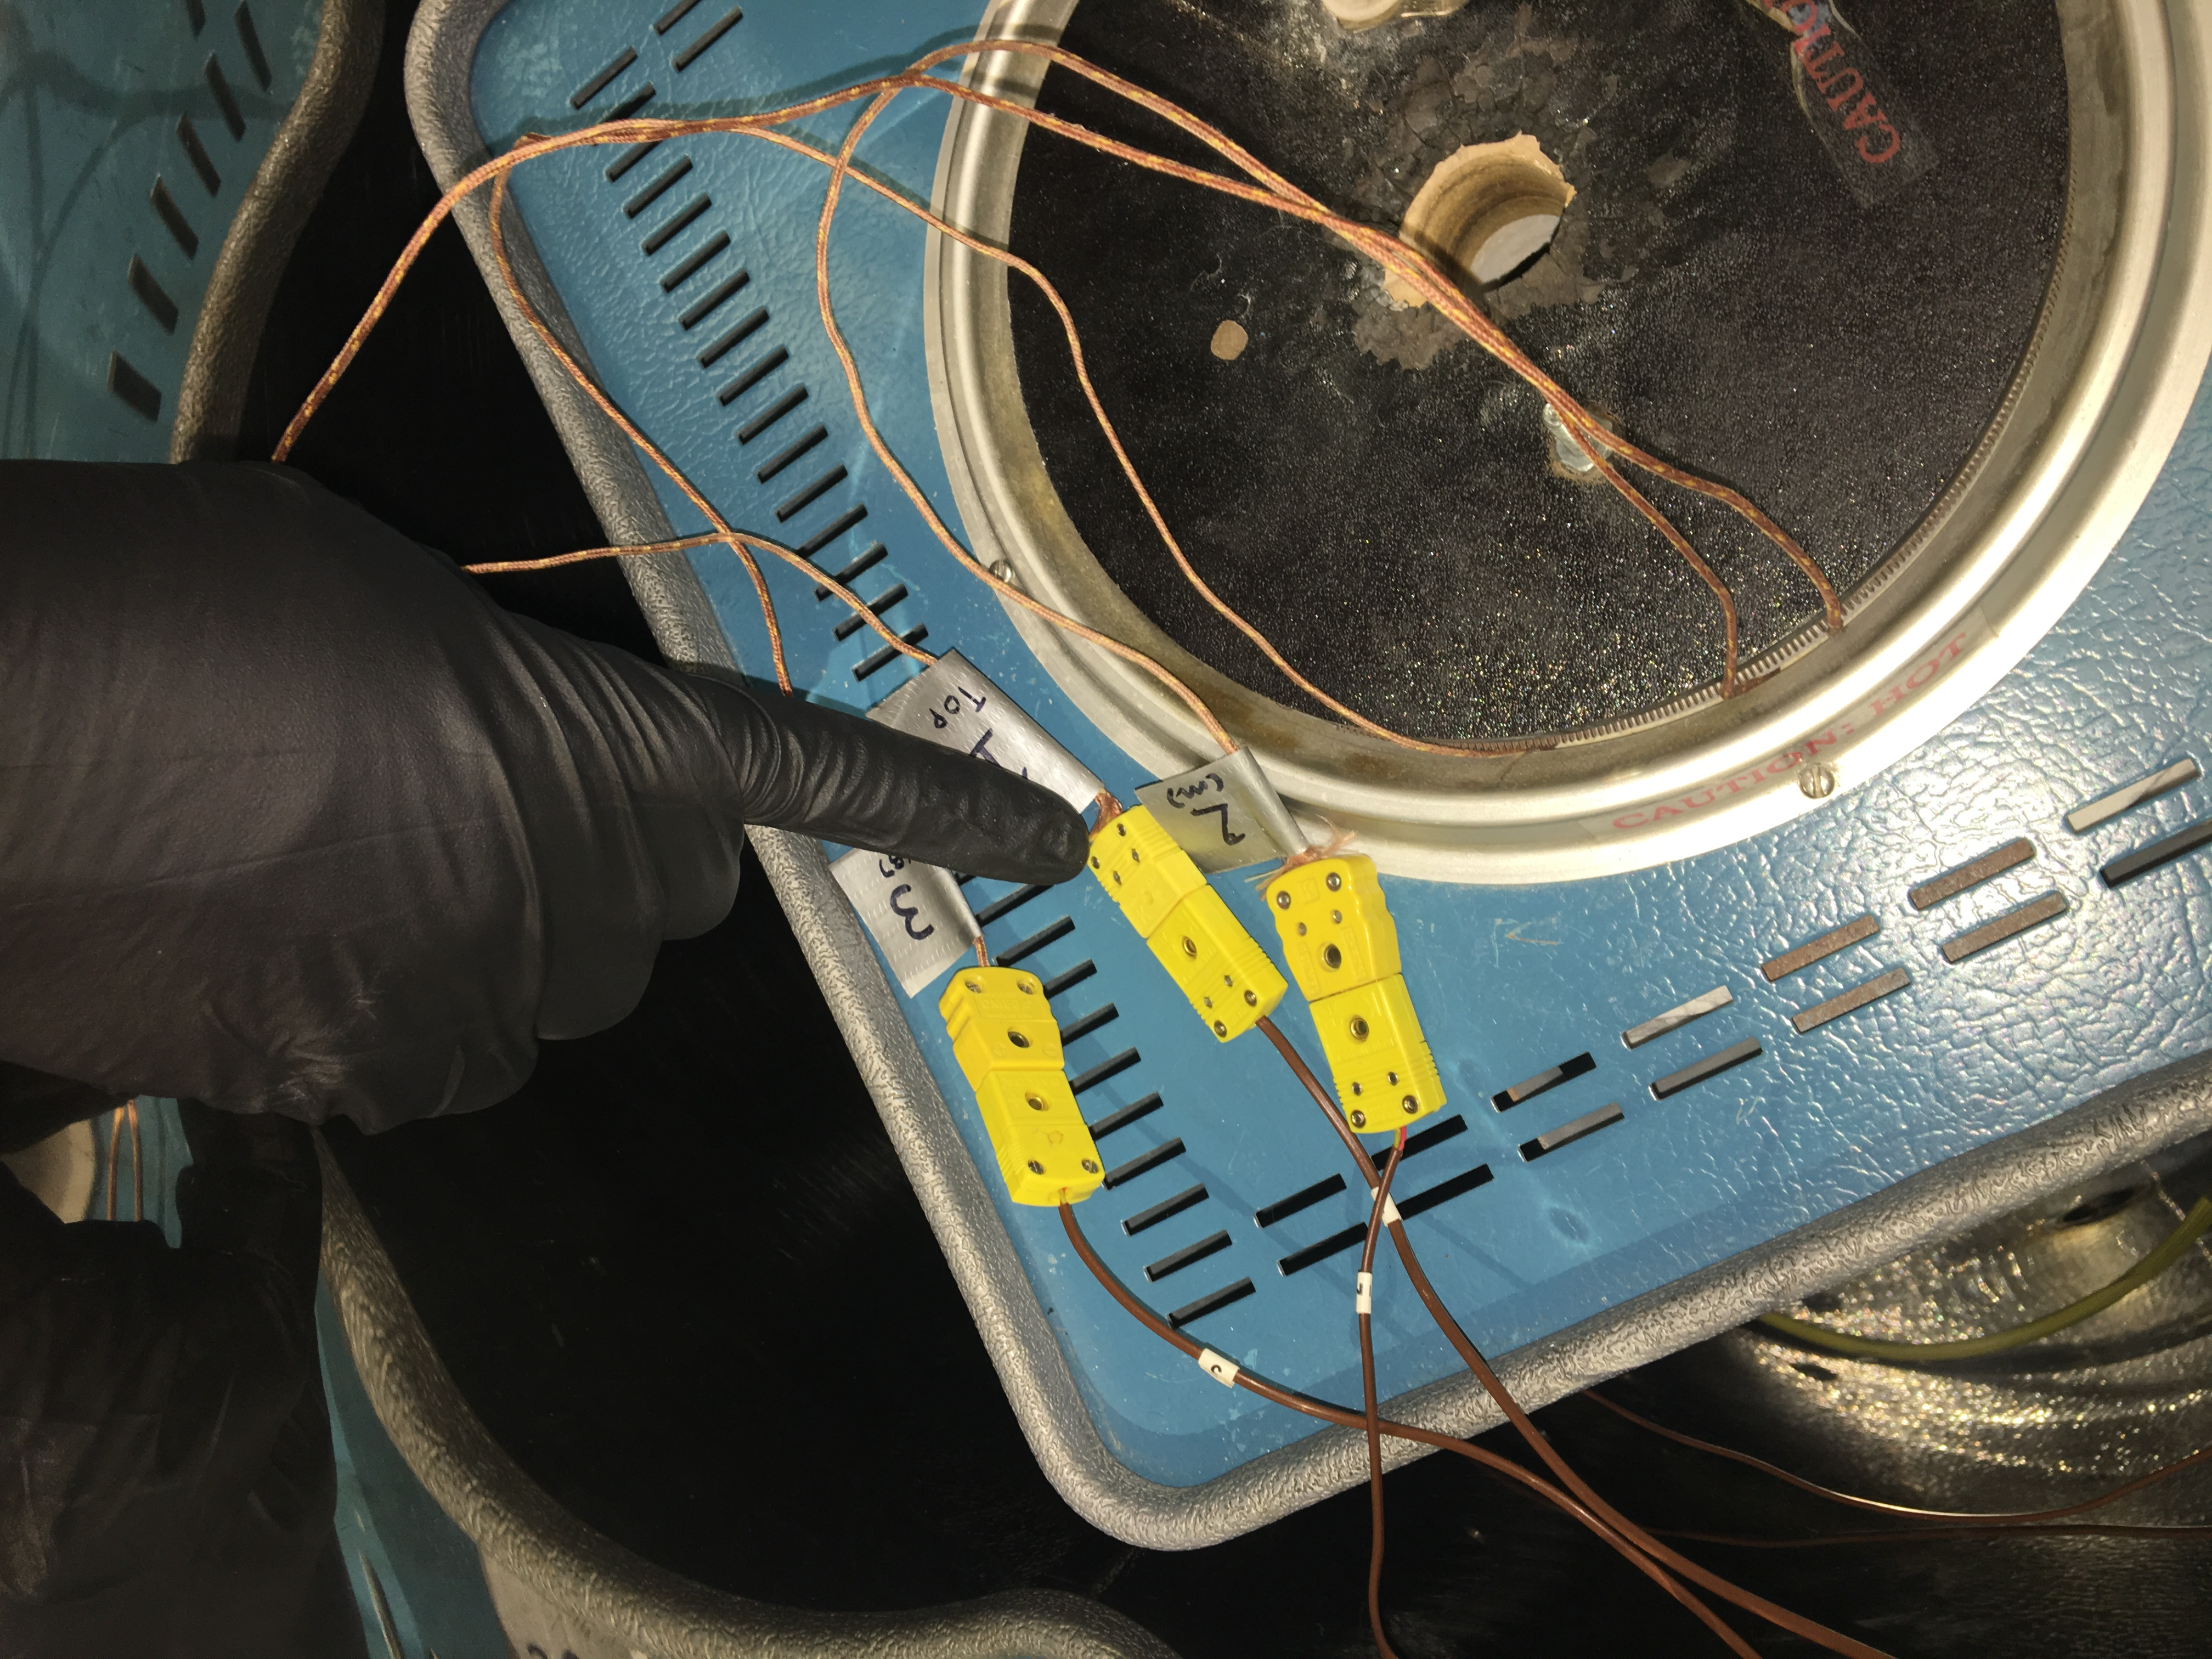
\includegraphics[width=.4\textwidth]{Thermocouples.jpg}
\caption{Thermocouple connections}
\label{fig:Thermocouples}
\end{figure}        
        
    \item Connect the TADA to the lab computer via the USB cable mounted 
        under the edge of the hood (see Figure \ref{fig:tada_connect})

        
\begin{figure}[H]
    \centering
    \subfloat[USB Connection]{{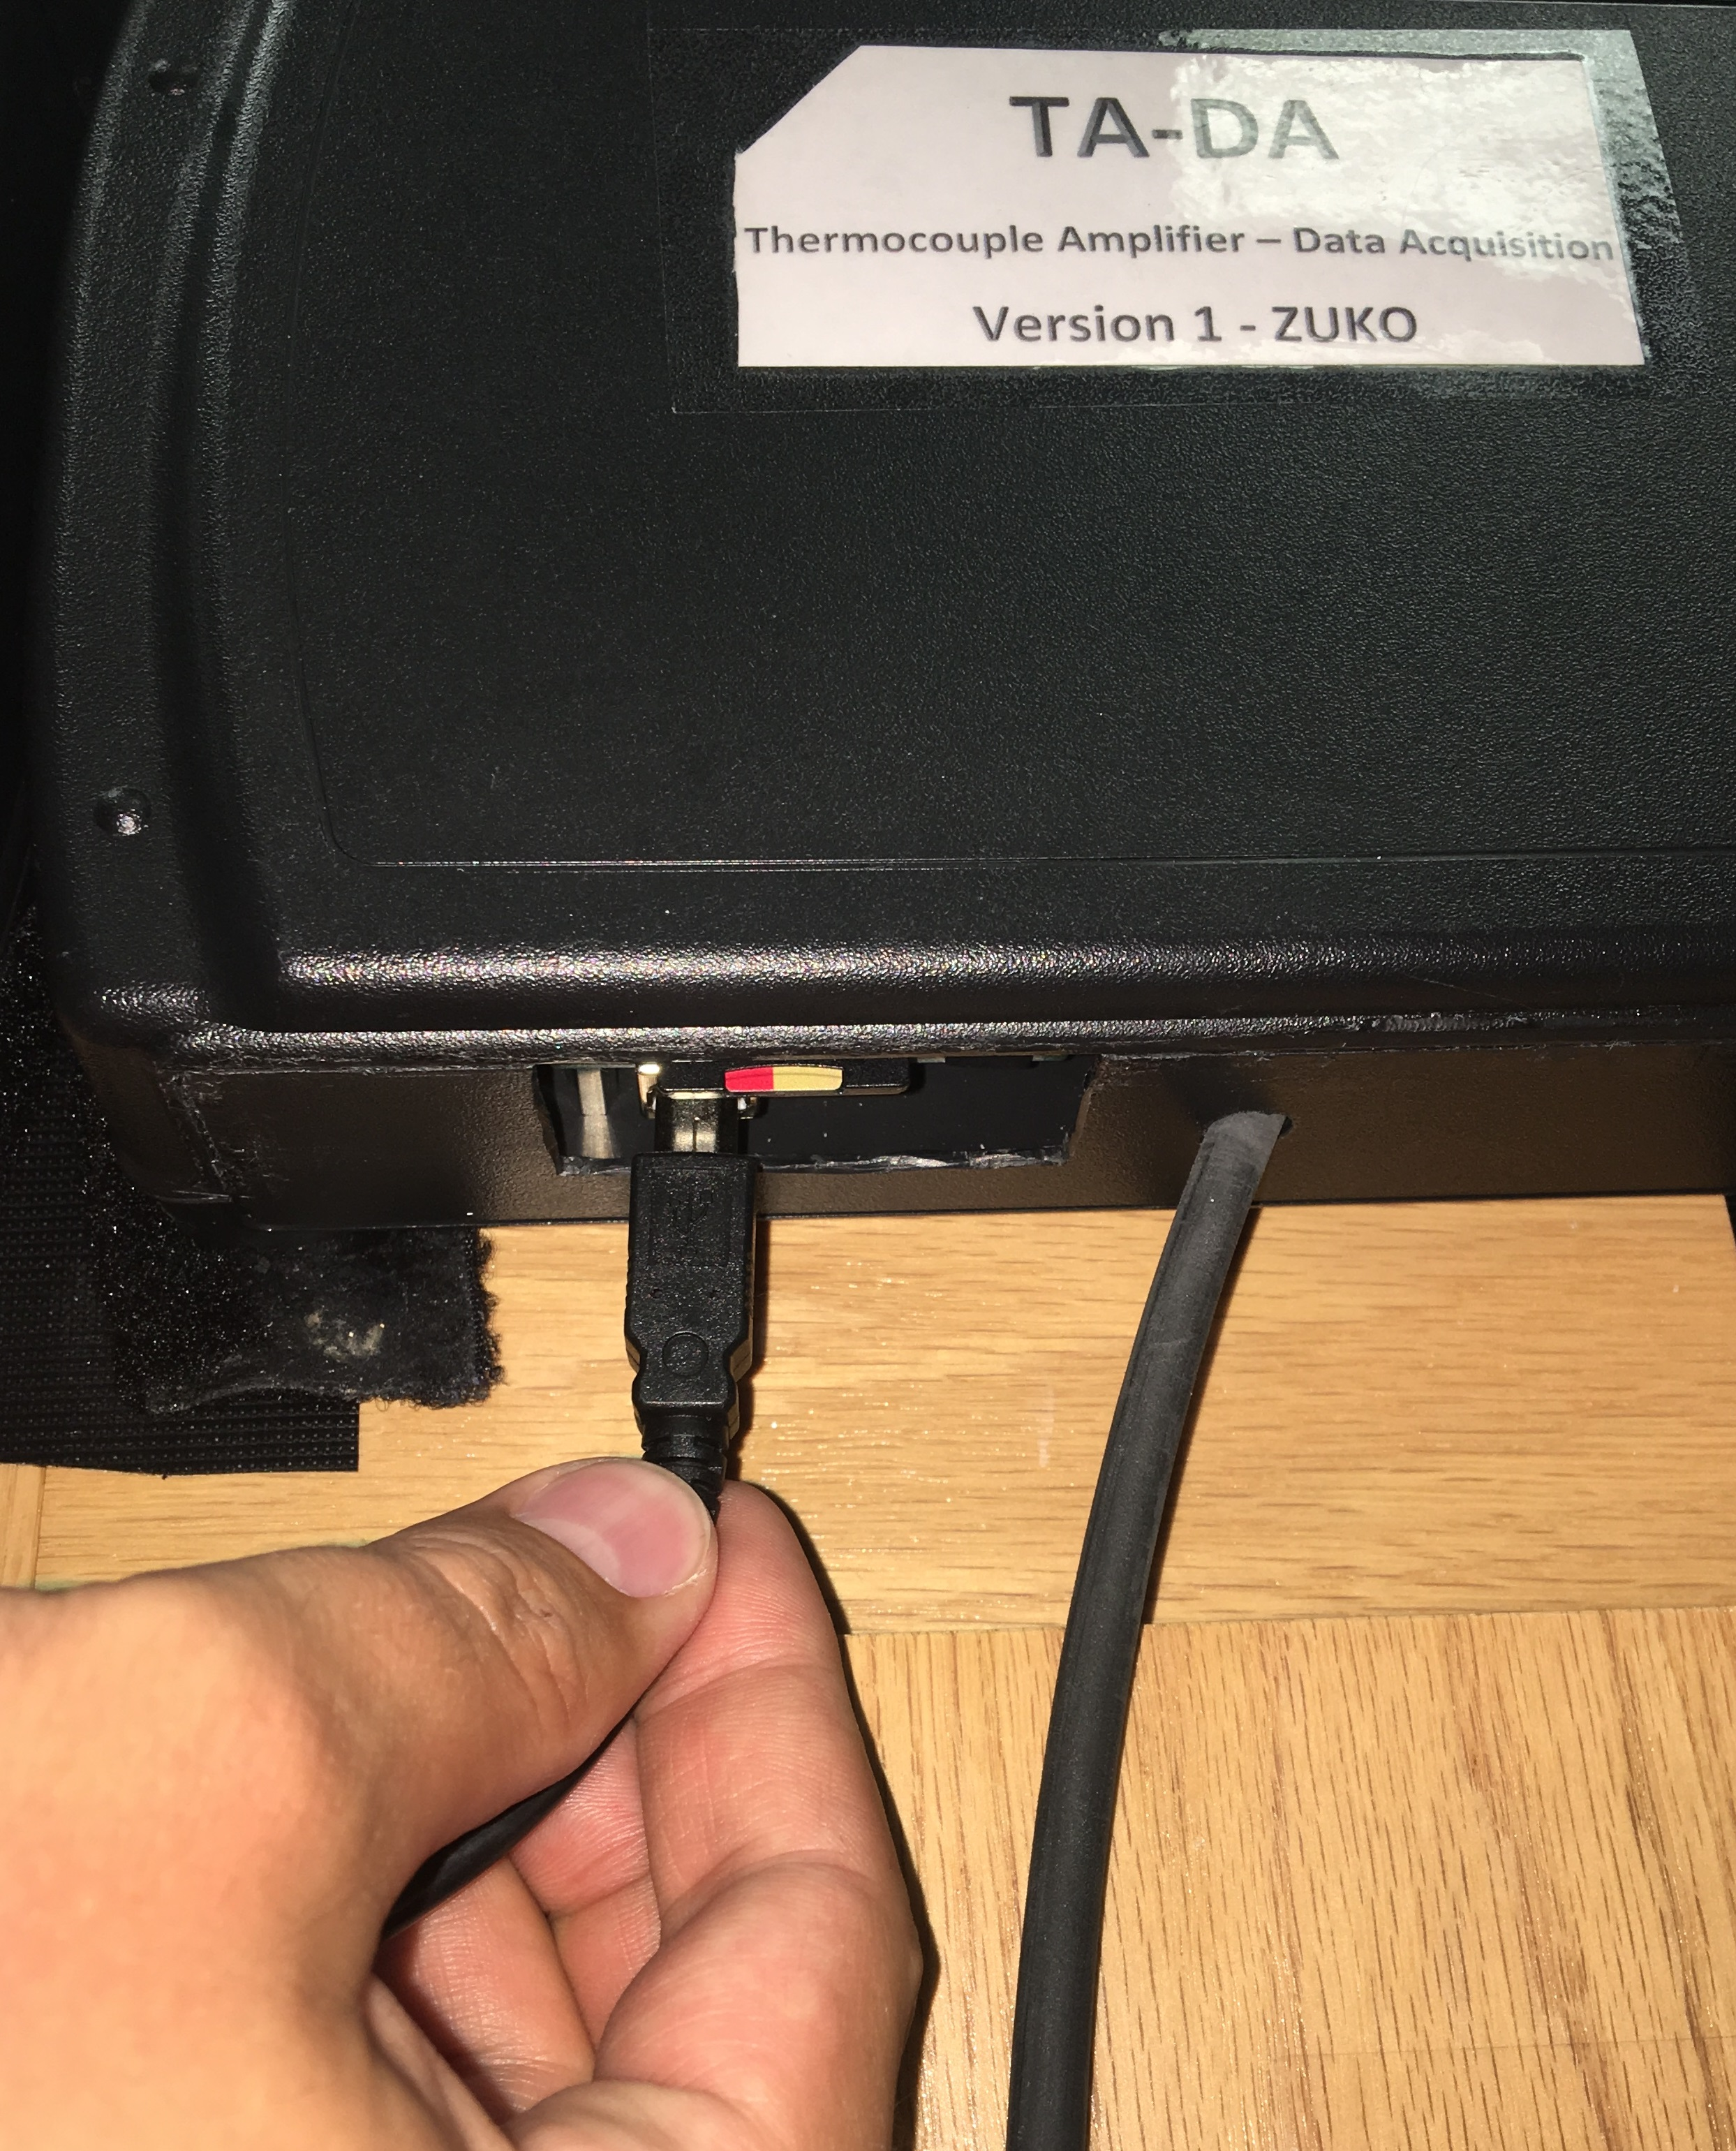
\includegraphics[height=5cm]{TADA_USB.jpg} }}
    \subfloat[24V Power Supply] {{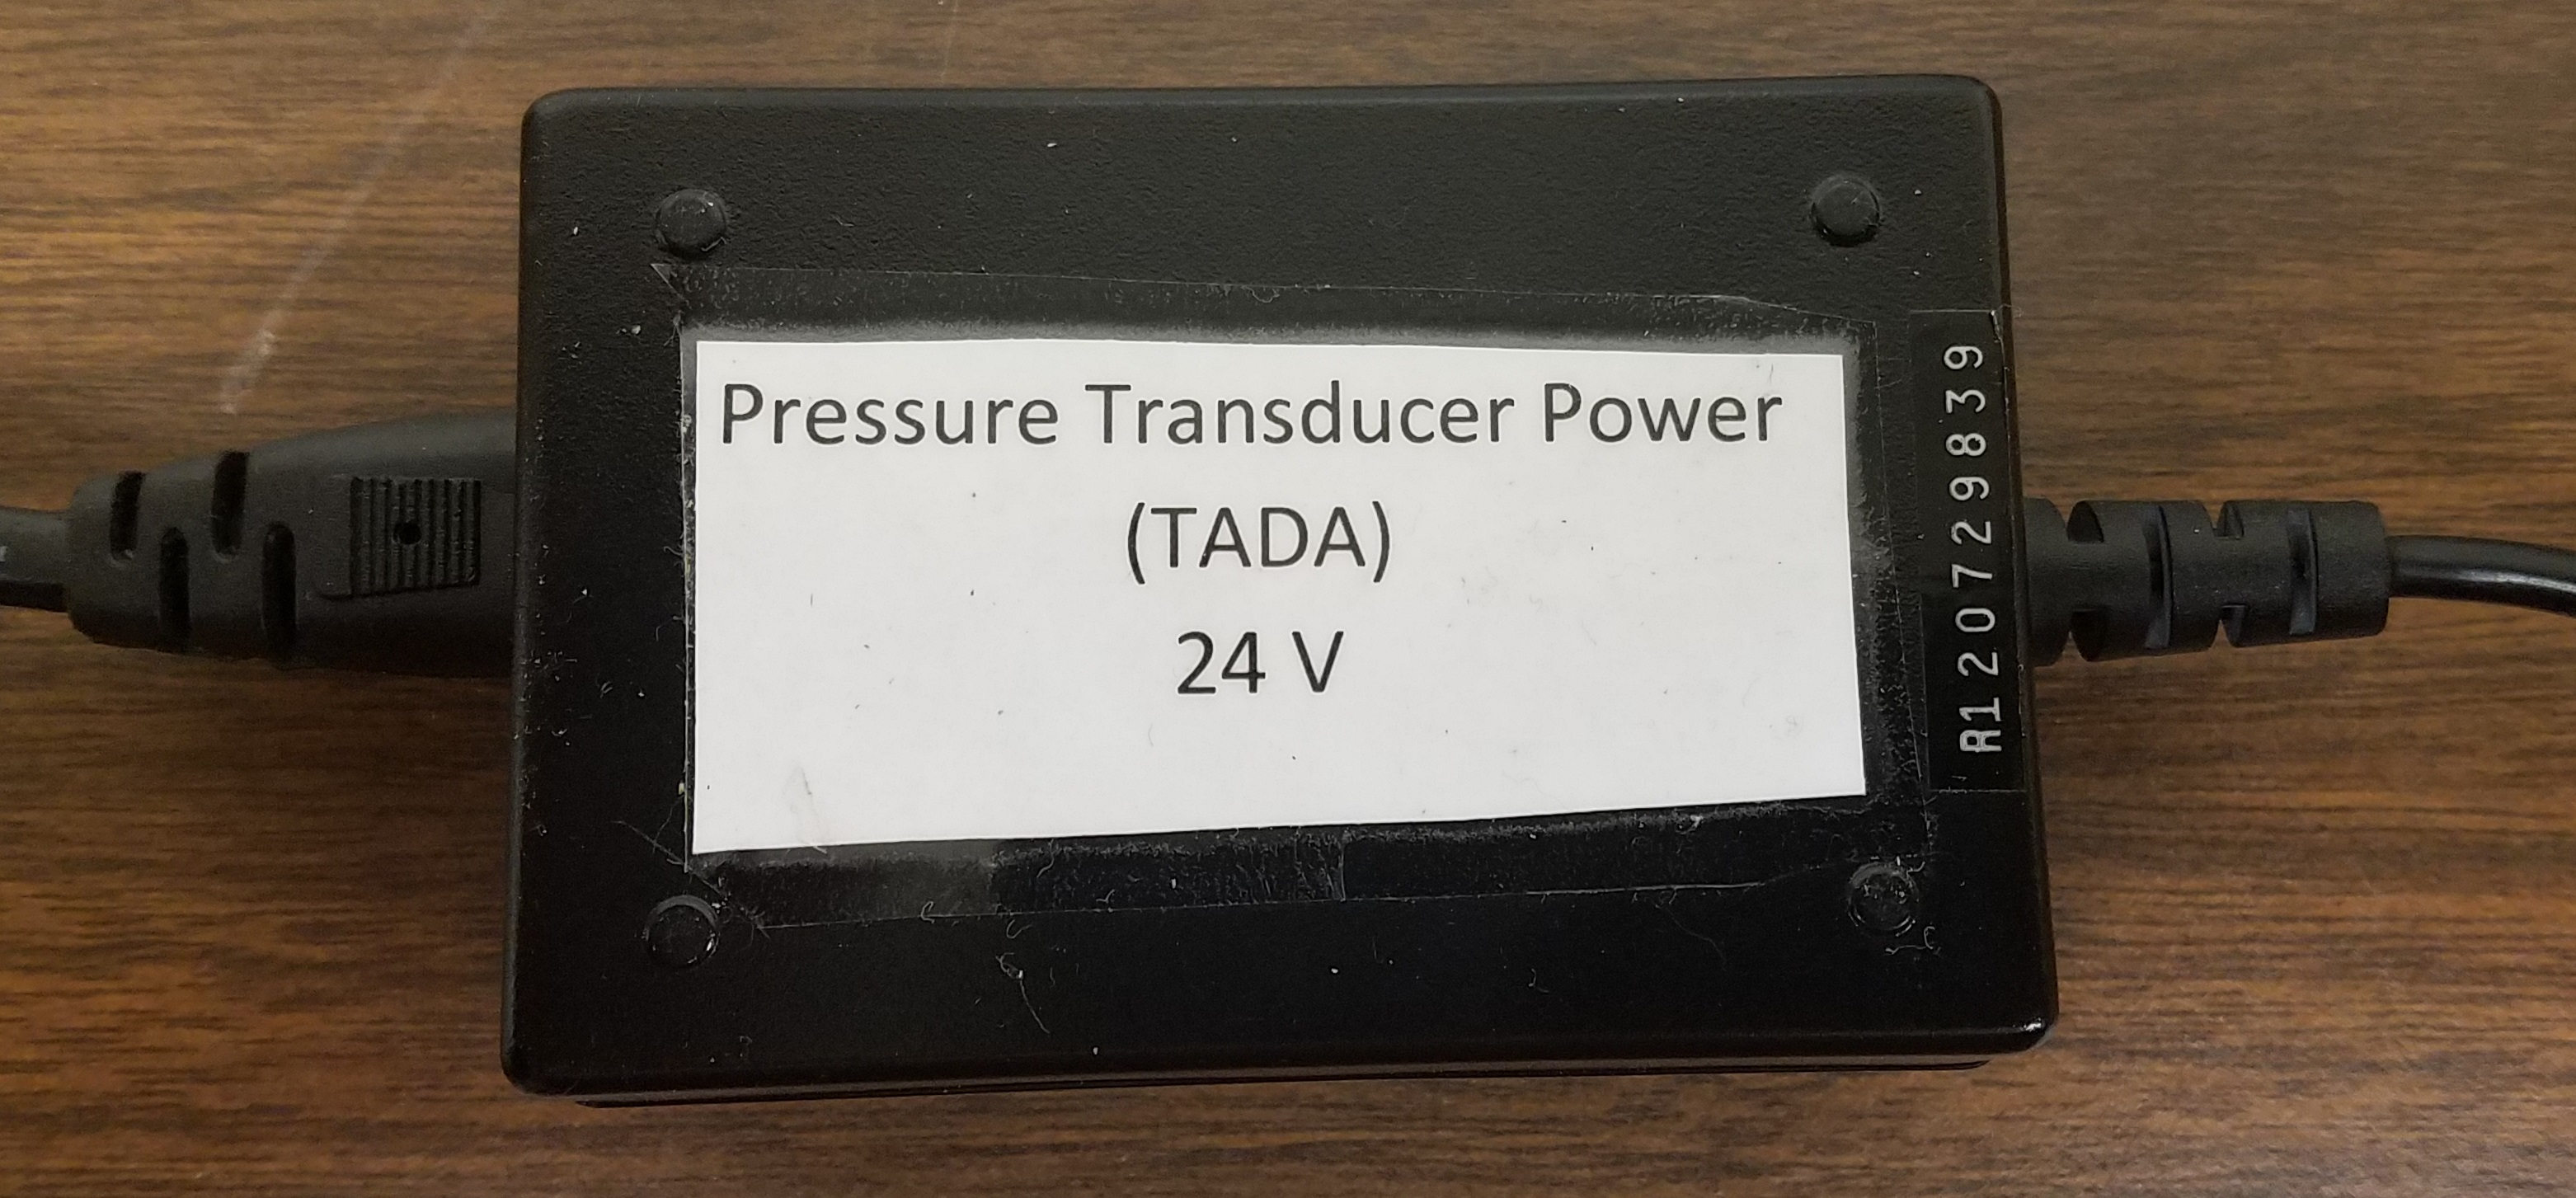
\includegraphics[height=5cm]{24v_powersupply.jpg} }}
    \caption{TADA Connections}
    \label{fig:tada_connect}
\end{figure}
        
    \item Plug in the wall power to the TADA 24-volt power supply (see Figure 
        \ref{fig:tada_connect})

    \item Open the TADA user interface program
            \begin{itemize}
            \item Path: \textit{C:\textbackslash Users\textbackslash  
                Public\textbackslash Public Documents\textbackslash AIT\textbackslash 
                ait\_exp\textbackslash TADA\textbackslash TADA\_UI.py}
            \item You may wish to make a shortcut to this location and put it on 
                your CAEDM desktop.
            \item The program will open two windows. Ensure both windows are 
                visible while using the program
            \item The serial communication LED in the TADA will start flashing
            \end{itemize}

\begin{figure}[H]
    \centering
    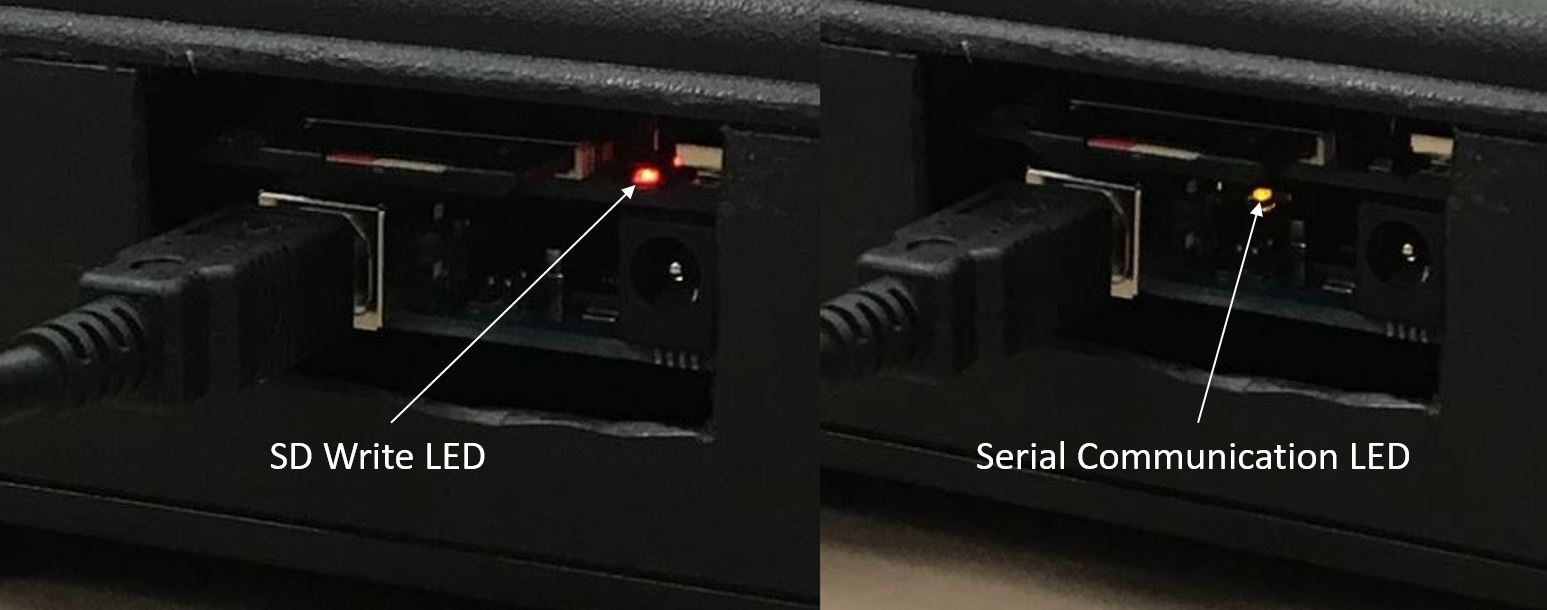
\includegraphics[width=.75\textwidth]{led_red_yellow.jpg}
    \caption{Control LEDs inside the TADA}
    \label{fig:tada_leds}
\end{figure}

    \item Twist both of the ARIA lead screws by hand such that the mounting 
        plate is all the way down and touching the base plate and the push block
        all the way back and is touching the horizontal stepper motor. (This is 
        the shutdown position. See Figure \ref{fig:shutdown_position})

\begin{figure}[H]
\centering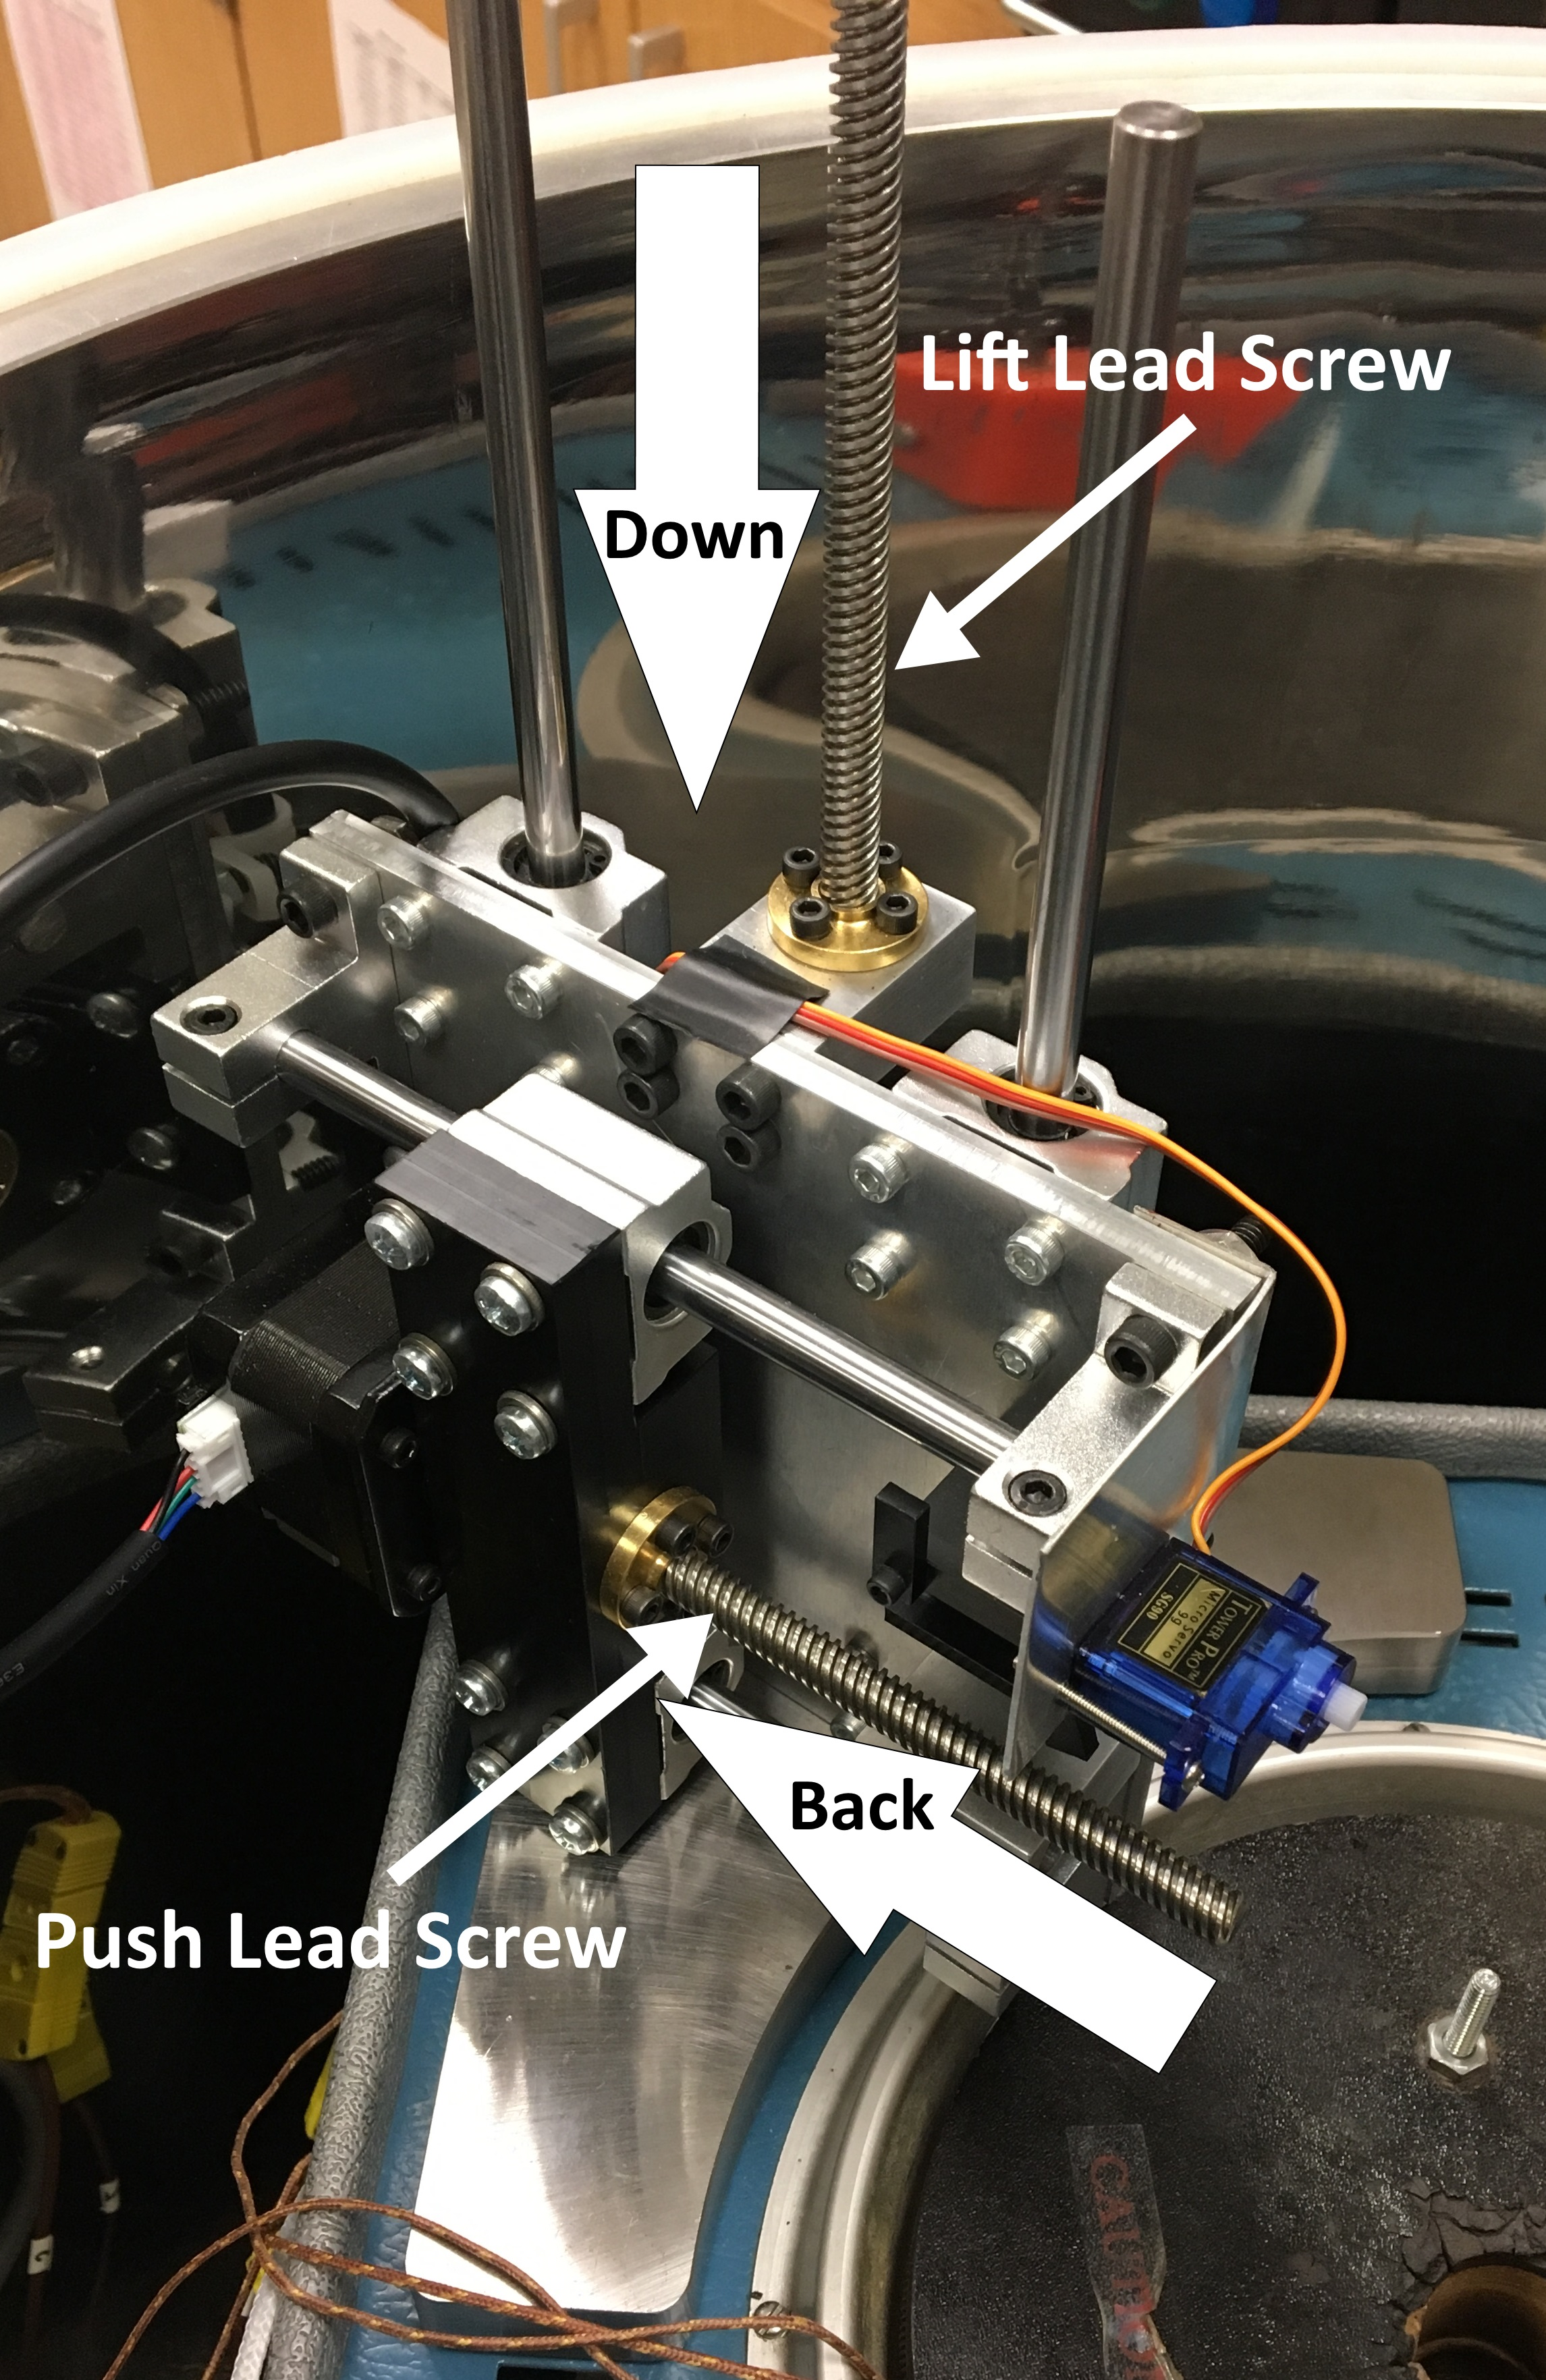
\includegraphics[width=.3\textwidth]{shutdown_position.jpg}
\caption{The shutdown position for the ARIA}
\label{fig:shutdown_position}
\end{figure}

    \item Ensure the three molex cables are securely plugged in to the ARIA 
        (see Figure \ref{fig:Molex_cables})
        \begin{itemize}
        \item Regardless of the experiments to be performed, ensure all three 
            are plugged in and the corresponding cables are not strained
        \end{itemize}
        
\begin{figure}[H]
\centering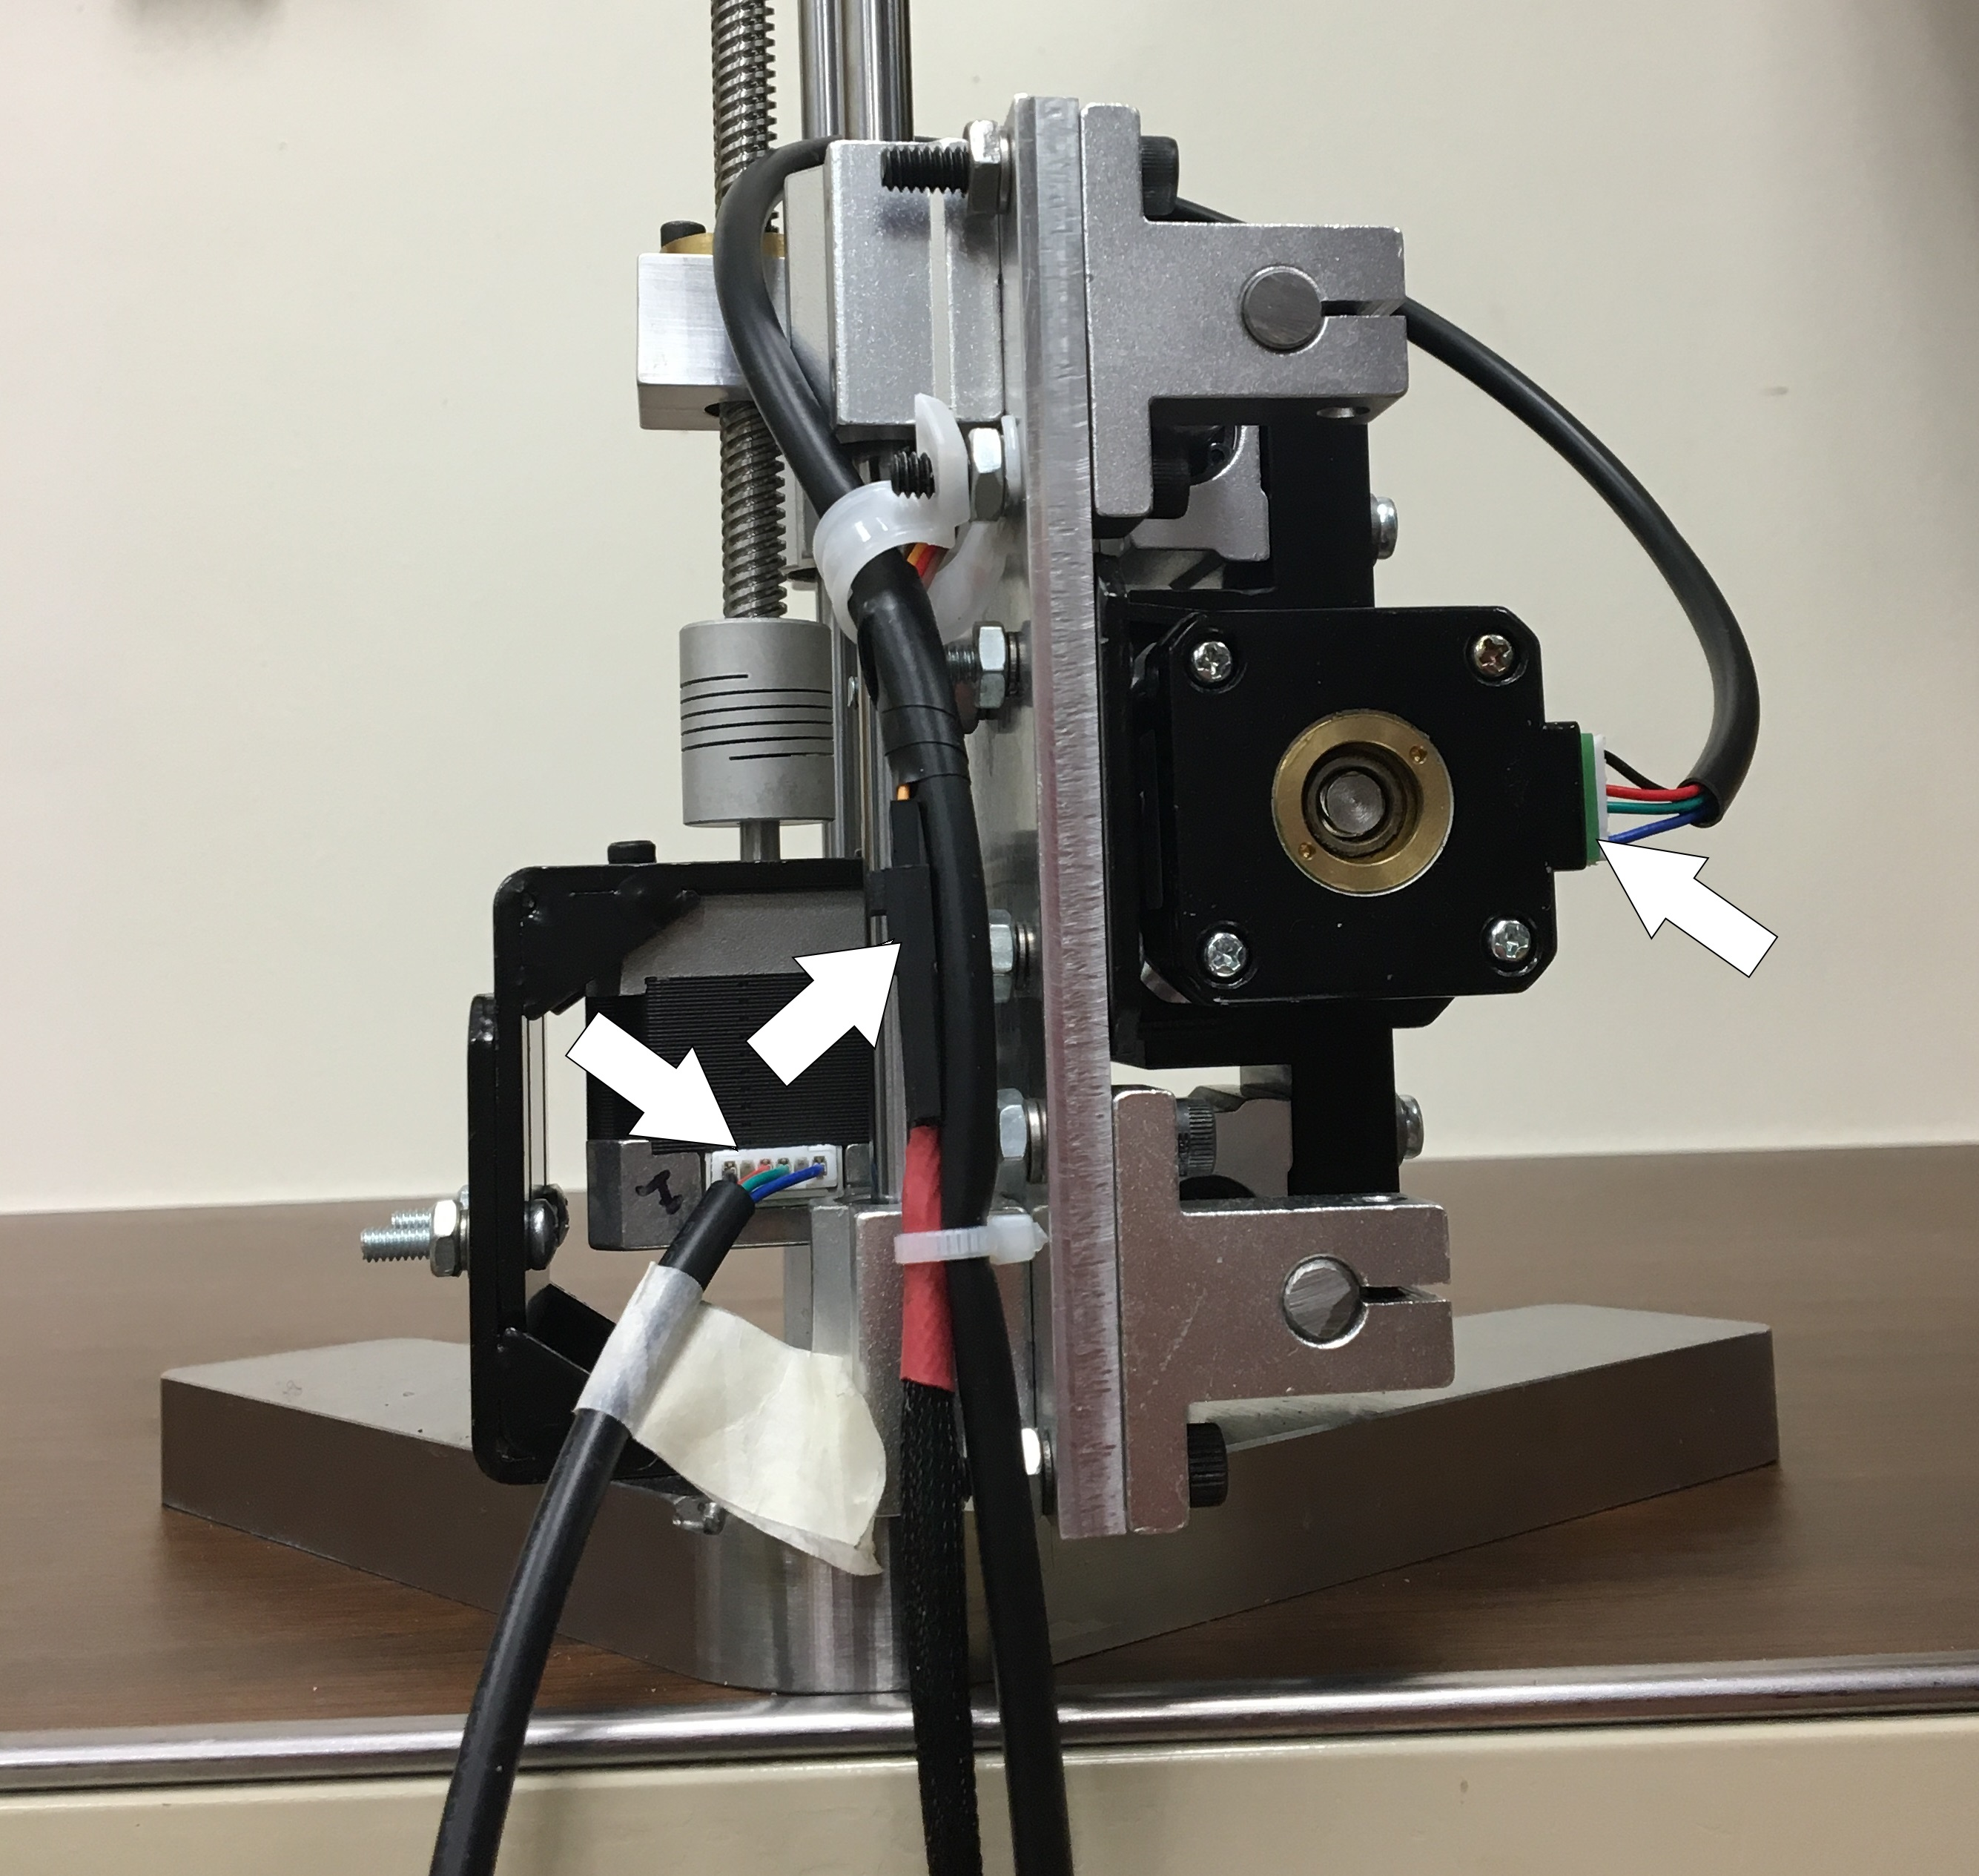
\includegraphics[width=.5\textwidth]{Molex_cables.jpg}
\caption{Molex cables secured and out of the way}
\label{fig:Molex_cables}
\end{figure}
    

    \item Plug 5 volt power supply into the ARIA control and wait for 
        initial setup sequence to complete (The two button lights on the ARIA
        control will come on when the sequence is complete) 
        (See Figure \ref{fig:5V_cable})
        
\begin{figure}[H]
\centering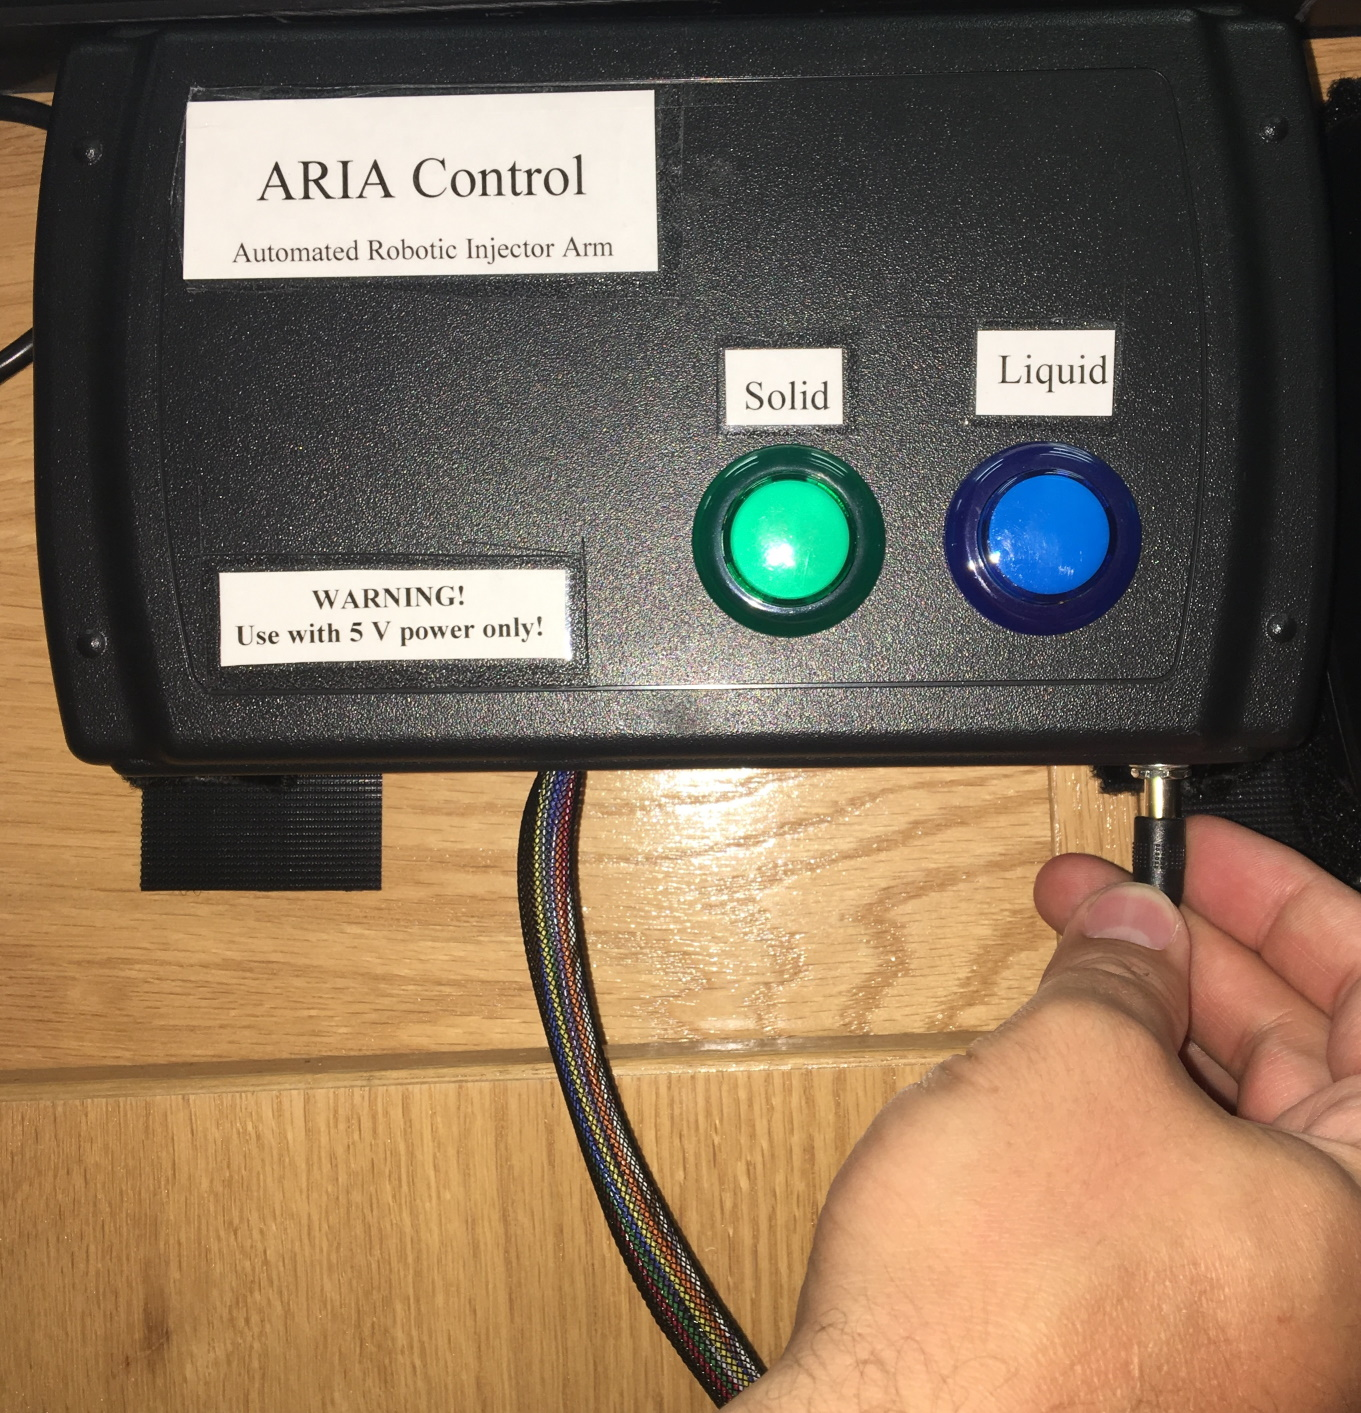
\includegraphics[width=.5\textwidth]{5V_cable.jpg}
\caption{Plug in ARIA; 5V ONLY}
\label{fig:5V_cable}
\end{figure}

    \item Test the placement of the ARIA using the funnel and ring stand
         \begin{itemize}
         \item Ensure the ring stand is secure in the ARIA, place the 
            funnel in the ring stand and run the solid program (Press the  
            "Solid" Button)
		 \item Note that the end of the ring stand rod must be nearly flush with the inside surface
             of the ring stand mount block (See Figure \ref{fig:flush_r_stand})
         \item If the funnel does not go directly into the flask, adjust the placement and retest 
            until properly positioned
         \end{itemize}
         
\begin{figure}[H]
\centering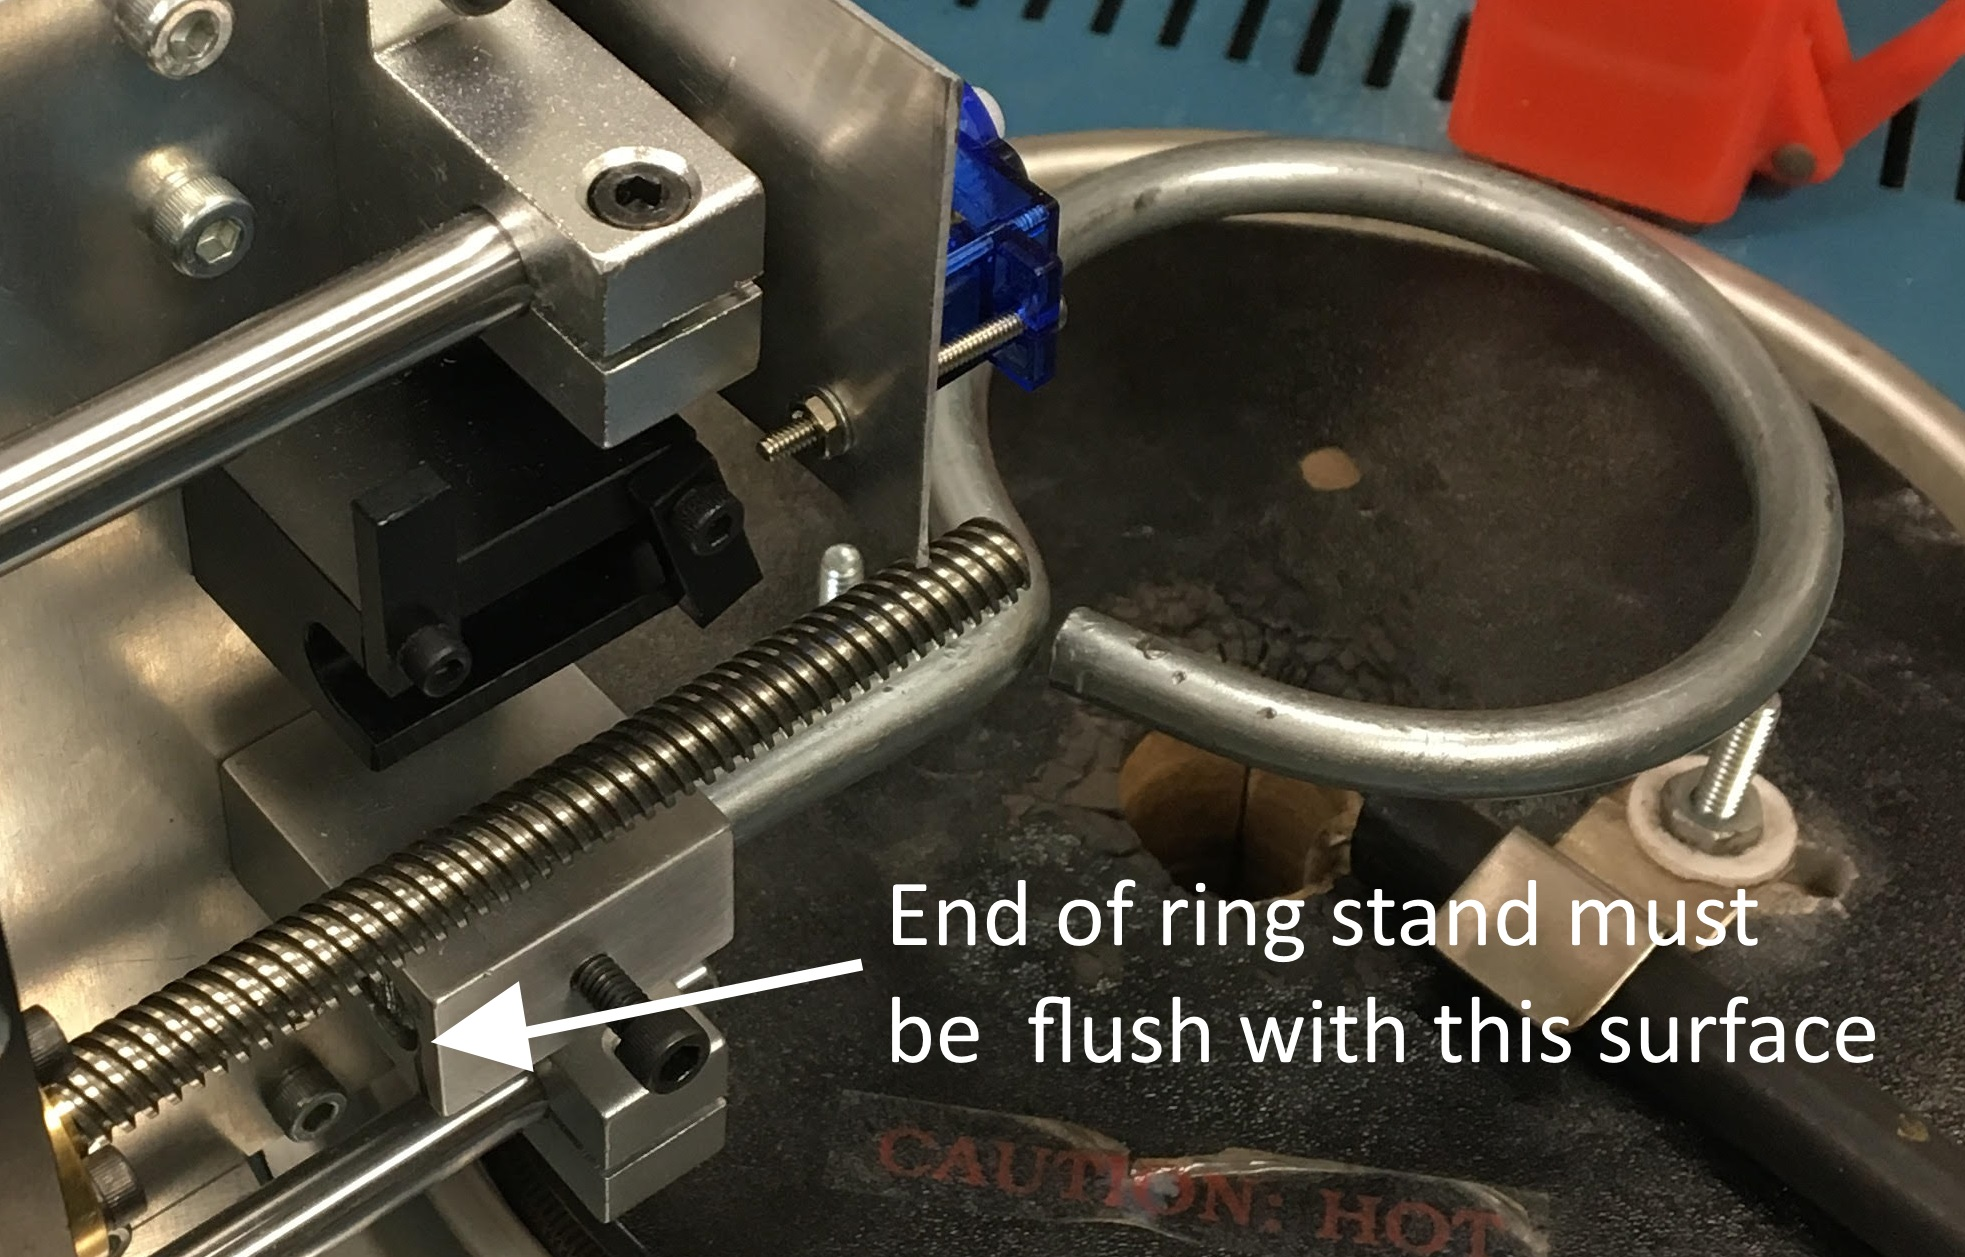
\includegraphics[width=.5\textwidth]{flush_r_stand.jpg}
\caption{Place the ring stand so its end is flush with the inside surface of the mount block}
\label{fig:flush_r_stand}
\end{figure}
         
    \item Test the placement of the mirror using the tablet and camera % SEE FIGURES
        \begin{itemize}
        \item Power on the tablet and connect it to the camera's Wi-Fi (See 
            Section \ref{sec:cam_tab} on how to do this)
        \item Open the Capture app to use the camera's view finder
        \item Mount the camera on the side of the furnace (See Section 
            \ref{sec:cam_on_furn})
           
        \item Using the camera's view finder on the tablet, adjust the
            position of the mirror on the furnace to align the camera's view to 
            see directly down the center of the flask
            \begin{itemize}
            \item The camera should be positioned so that the hole in the 
                furnace and the mirror are visible 
            \end{itemize}
        \item Once you have aligned the mirror, remove and shutdown the camera 
            for initial furnace heating
        \end{itemize}

    \item Once the target temperature is reached, allow the system to come to 
        equilibrium
        \begin{itemize}
        \item The "Temp Ready" indicator in the TADA\_UI window should turn 
            green when the system has come to an acceptable equilibrated state
        \end{itemize}
    \end{enumerate}

    
\subsection{Experimental}
This section outlines the steps for experimental runs. Each experiment should be
performed following these steps exactly (insofar as that is possible). Doing so
will ensure consistent results with the lowest uncertainty possible.

\textbf{
Before beginning experiments, ALL operators ensure they are using
appropriate PPE for handling chemicals (e.g. nitrile gloves and splash goggles)
and have minimized laboratory hazards}

\begin{itemize}
\item Ensure your workspace, the area around the computer and 
    both hoods are free of clutter, tripping hazards or any object 
    which could present a hazard to you or anyone else in the lab
\item Refer to the SDS for the chemical you are working 
    with when determining appropriate PPE
    \begin{itemize}
    \item NOTE: Some SDS's will recommend using a face shield in 
        addition to splash goggles when handing their respective 
        chemicals. In our lab we will use ventilation hoods which, 
        when used properly, serve as better protection than face 
        shields. Therefore, any time an SDS recommends using a 
        face shield you may safely ignore that recommendation 
        provided you are using the hood properly by positioning the 
        sash between your face and the work being performed in 
        the hood.
    \end{itemize}
    
\item Unless an SDS states otherwise, lab coats are recommended but 
    not required when handling chemicals
\item All chemical handling (except for injection into the furnace) 
    should be done in the hood to avoid a potential fire hazard 
\end{itemize}


    \begin{enumerate}
    
    \item Measure out sample
        \begin{itemize}
        \item Liquids
            \begin{itemize}
            \item Take 2 clean 100 ml beakers and put them in the hood (these will be your sample
                    and waste beakers)
            \item Place a small amount of compound into the sample beaker
            \item Rinse the syringe of any extraneous compounds 3 times
                \begin{itemize}
                \item Draw approximately 300 microliters into the syringe from 
                    the sample beaker and
                    eject it into the waste beaker
                \item This only needs to be done once a day
                \end{itemize}
            \item Draw sample amount into a right-angle syringe
                \begin{itemize}
                \item Begin by drawing an excess amount of compound into the syringe
                \item Draw slowly to minimize air bubbles in the syringe
                \item Hold syringe vertically to move air bubbles to the top, gently tapping the 
                    syringe if necessary
                \item Gently eject the syringe into the waste beaker to remove any air bubbles until
                    the syringe reads the desired amount
                \item The desired amount should not exceed 250 microliters
                \end{itemize}
            \end{itemize}

        
        \item Solids
            \begin{itemize}
            \item Tare the lab scale with the weigh boat and measure out sample
                \begin{itemize}
                \item This should not exceed 250 mg
                \end{itemize}
            \end{itemize}
            
        \item Gases
            \begin{itemize}
            \item Draw sample amount into a right-angle syringe  
                \begin{itemize}
                \item This should not exceed 250 microliters
                \end{itemize}
            \end{itemize}
            
        \end{itemize}

     \item Secure the sample to the ARIA
        \begin{itemize}
        \item Liquid/Gases Sample
            \begin{itemize}
            \item Place the syringe securely into the syringe holder on the 
                ARIA, making sure the tip of the syringe is aligning down the 
                center of the hole in the funnel
                needle is aligned down the center of the hole in the furnace
			\item Test placement one more time with the opposite program (for 
                liquid sample use the solid button)
            \end{itemize}
            
        \item Solid Sample
            \begin{itemize}
            \item Carefully insert the weigh boat into the weigh boat holder and
                press the weigh boat holder onto the servo shaft so the weigh 
                boat is in a near-horizontal position
			\item Test placement one more time with the opposite program (for 
                solid sample use the liquid button)
            \end{itemize}
            
        \end{itemize}
            
    \item Remove gloves before proceeding
	\item Ensure the camera has sufficient battery and is powered on
        \begin{itemize}
        \item Reconnect the camera to the tablet if necessary
        \end{itemize}
    \item Secure the camera to the side of the furnace


    
    \item \textbf{Simultaneously} remove the snorkel from inside the vessel and 
        place above the rupture 
        disk (see Figure \ref{fig:rupture_hood}) \textbf{and} place lid on 
        pressure vessel and secure in place with the clamps and cable

\begin{figure}[H]
\centering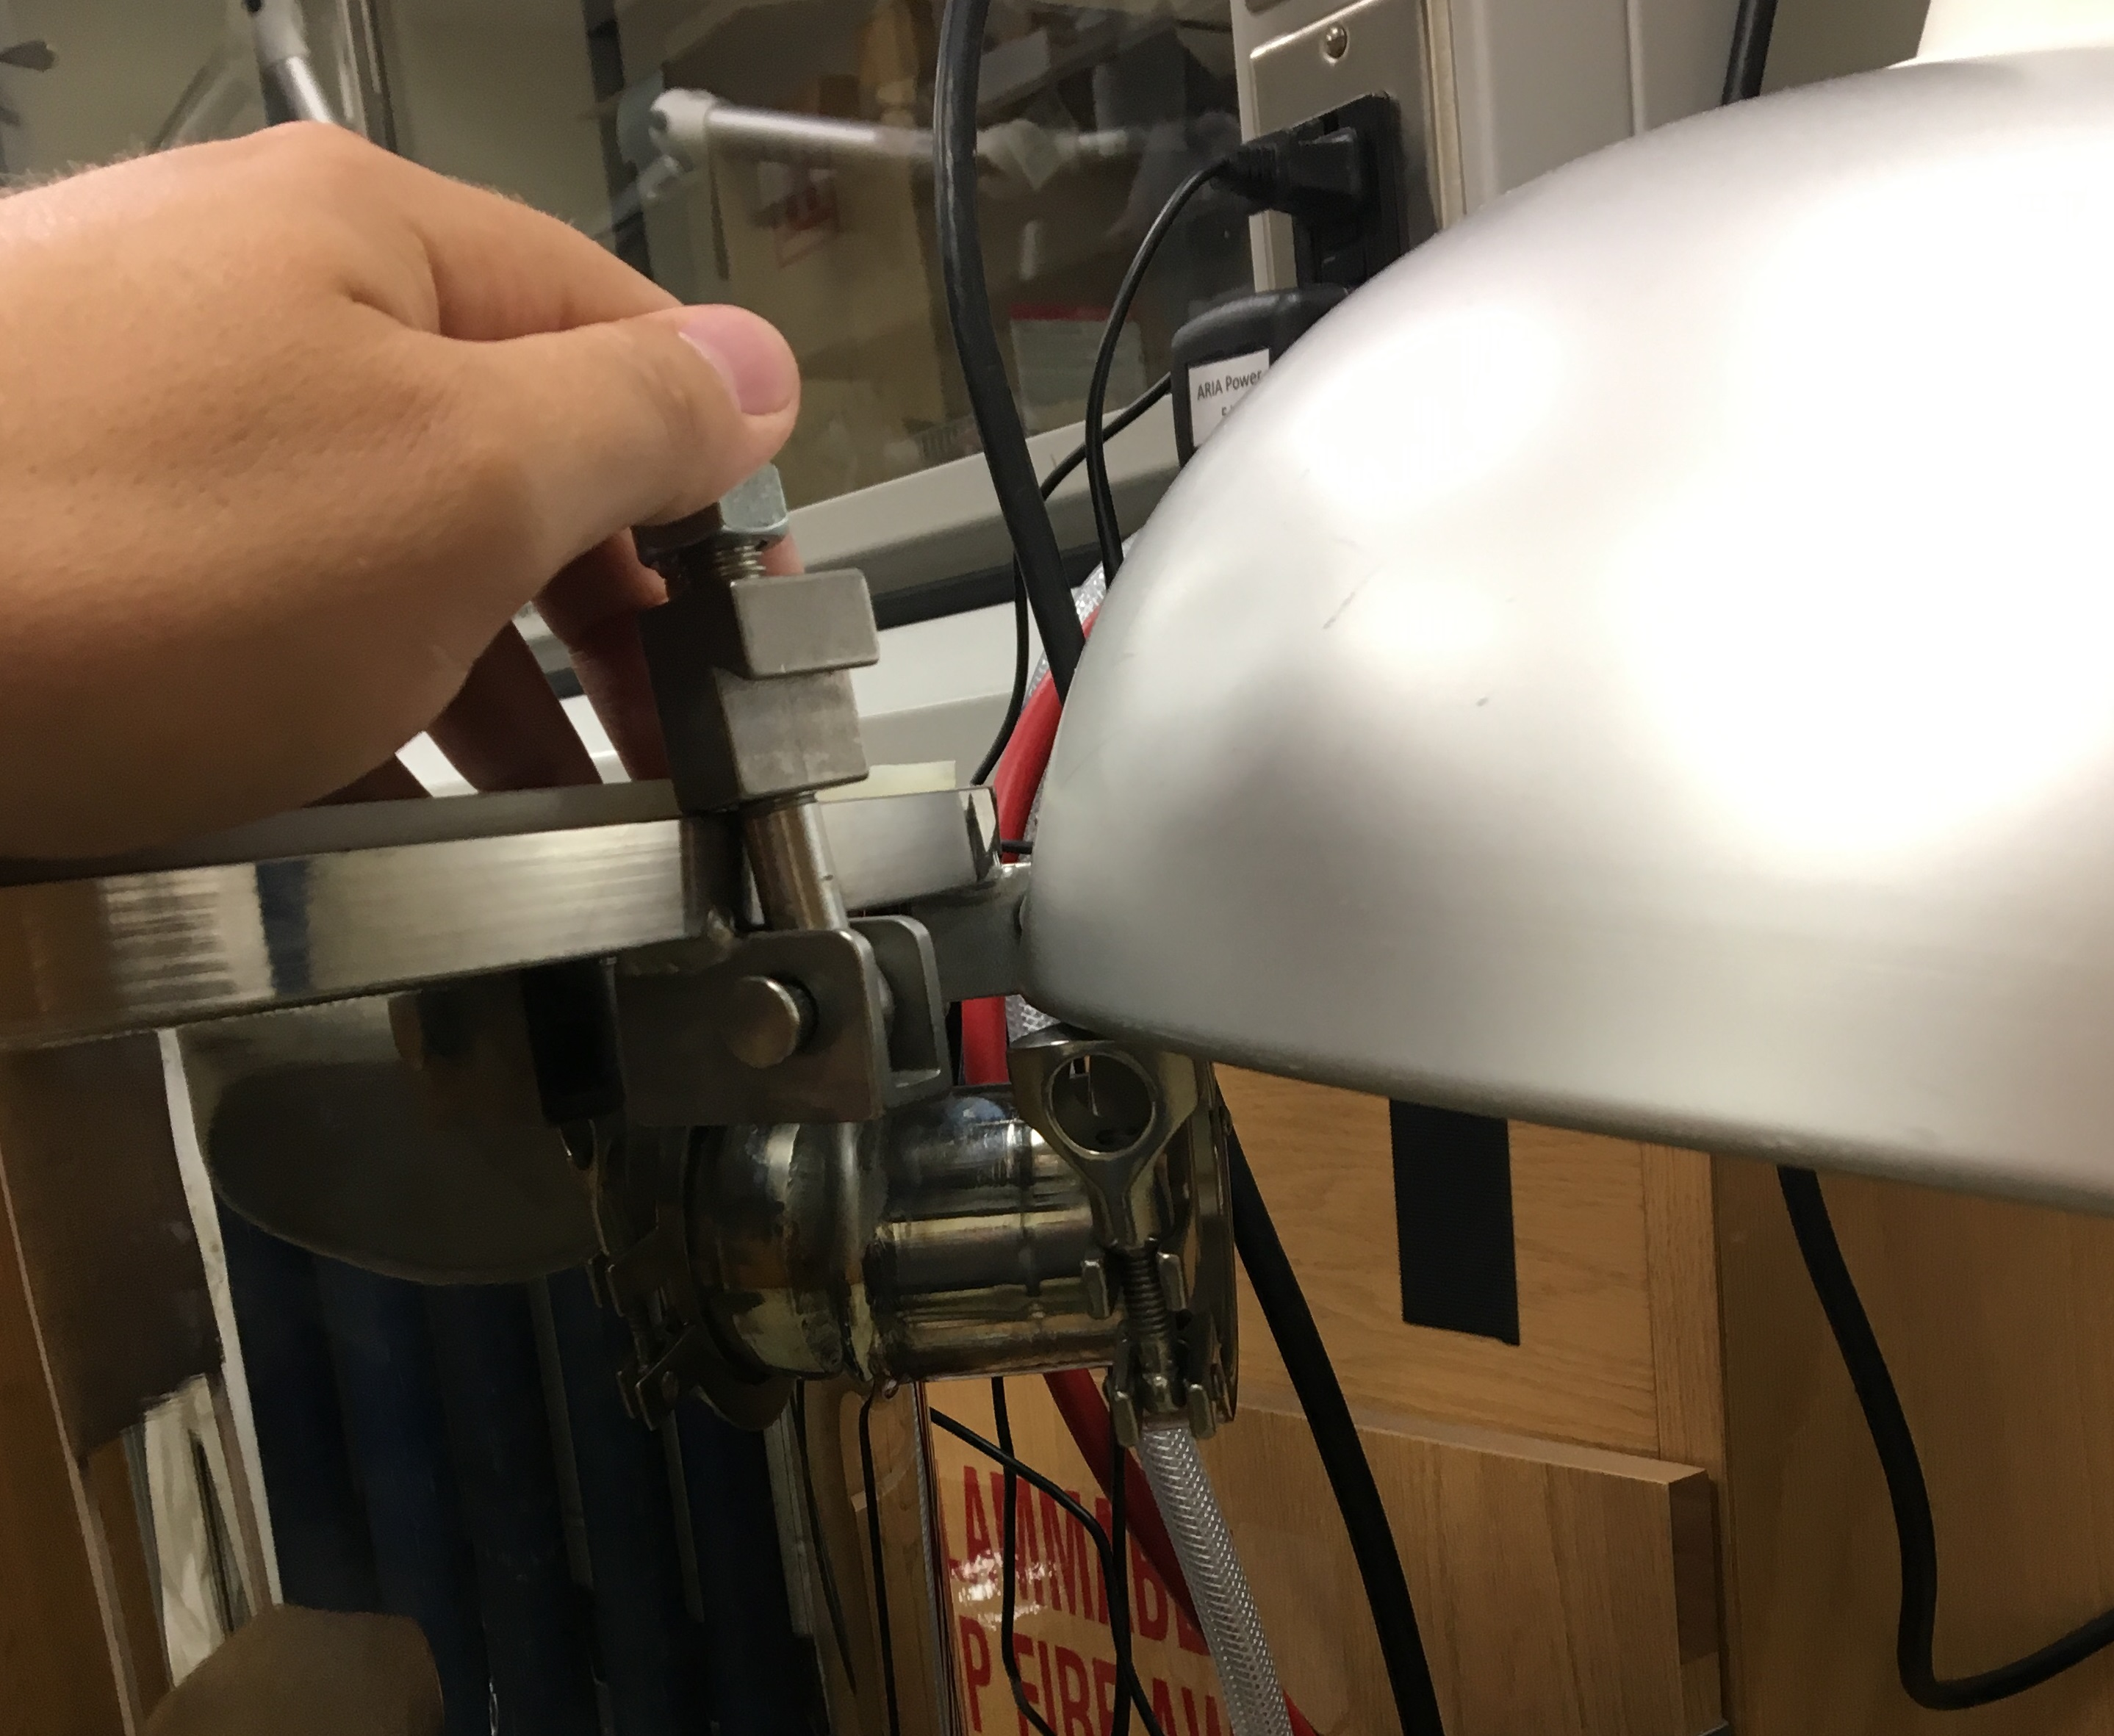
\includegraphics[width=.3\textwidth]{rupture_hood.jpg}
\caption{Snorkel placement during operation}
\label{fig:rupture_hood}
\end{figure} 

        \begin{itemize}
        \item Two people should perform this step. One to remove the snorkel
            and the other to place the lid
        \item Open the sash on the hood and carefully pull out the vessel lid 
            ensuring the outlet 
            hose does not catch on anything (do not pull it through the 
            sliding doors)
        \item When placing the lid, hold the lid directly above the vessel and 
            carefully lower it straight down on the vessel to avoid hitting the
            ARIA with the lid. Make sure to avoid crimping the outlet hose and 
            keep it as smooth and straight as possible
        \item Line up the two marks on the lid with the corresponding marks 
            on the vessel
        \item Ensure the lid is centered on the vessel by running your fingers
            around the edge to ensure the edge of the vessel and the lid are
            flush 
        \item Check that the lid lies flat on the O-ring and no wires or debris 
            will break the seal
        \item Hand tighten all the pressure vessel clamps on the lip of the lid 
            so the slack is taken out
        \item Using your other hand to keep the pressure vessel from rotating, 
			tighten the clamps in opposing pairs following the numbering on 
            the back of each clamp (See Figure \ref{fig:sec_lid}) using a 
            torque wrench, tightening each clamp until the torque reads 
            60 inch pounds
            \item Tighten each clamp again with the torque wrench, this time by 
            going around the circle, ensuring that torque is 60 inch pounds on 
            each.
        \item Loop the safety cable through both lid handles and through the 
            handles on both sides of the vessel and then back through the lid 
            handles so the two ends meet then secure the two ends together 
            (See Figure \ref{fig:sec_lid})

\begin{figure}[H]
    \centering
    \subfloat[Clamp numbering]{{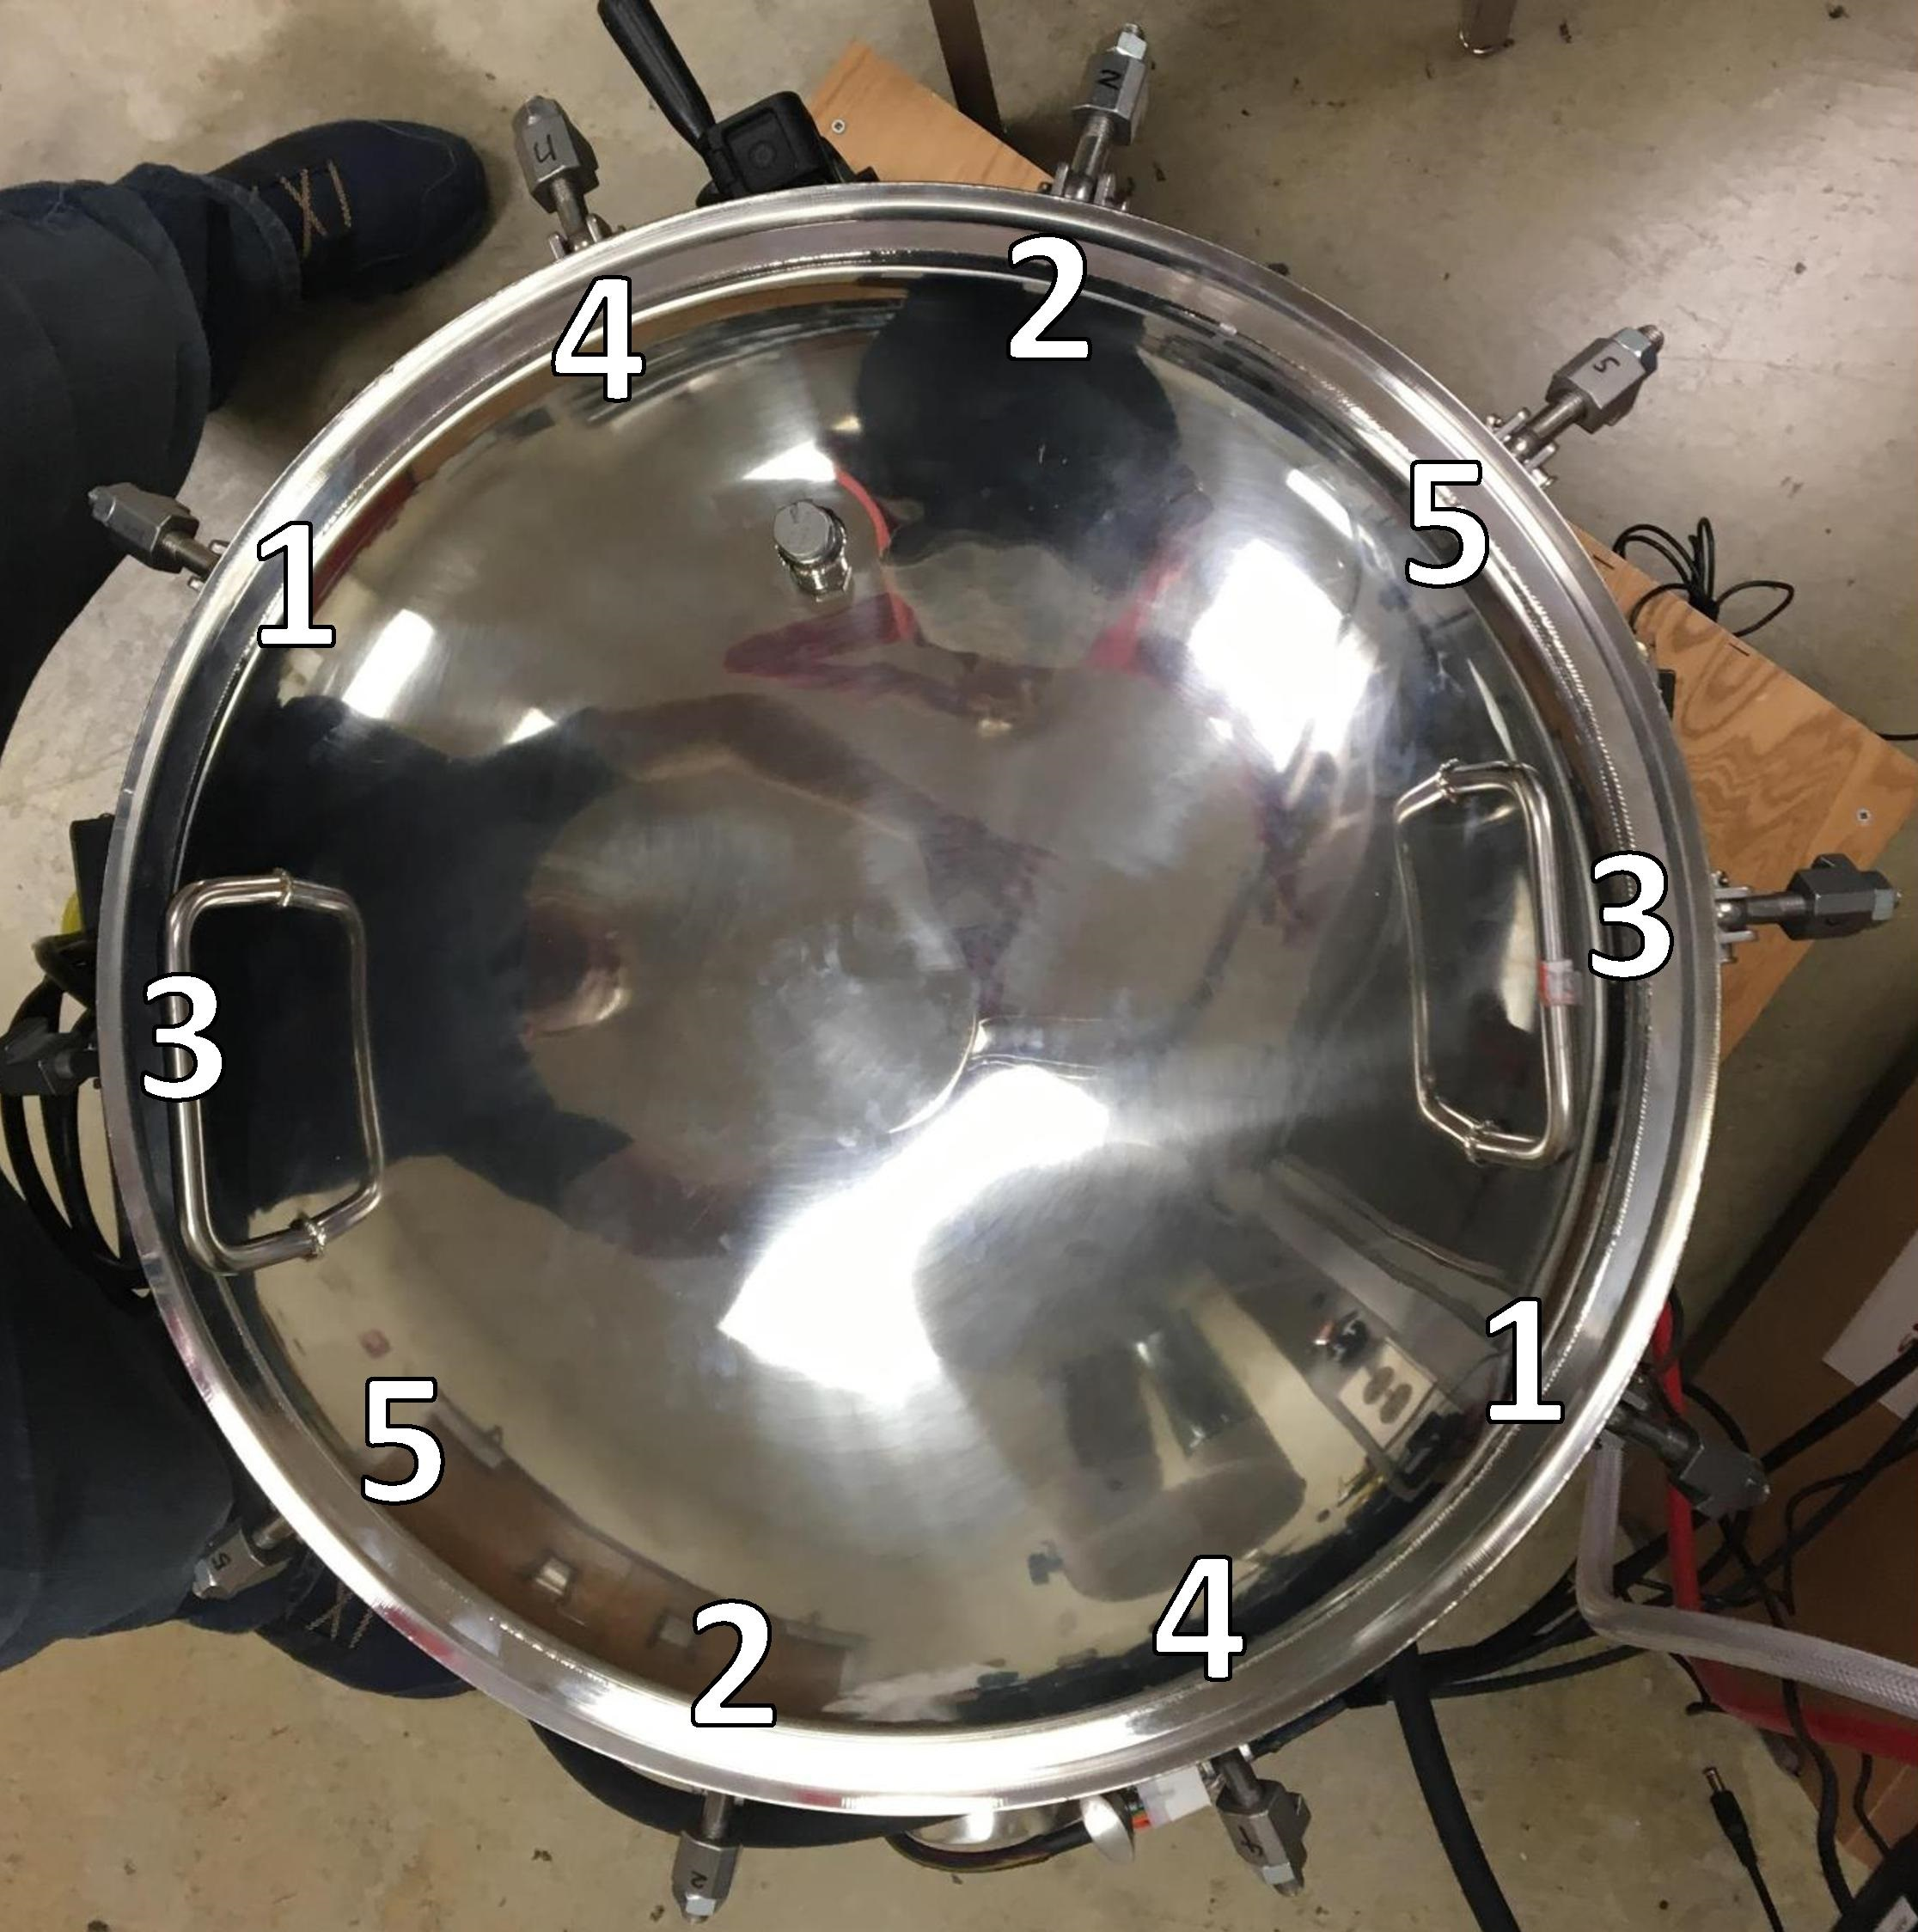
\includegraphics[height=8cm]{Top_of_lid.jpg} }}
    \subfloat[Safety Cable Installation] {{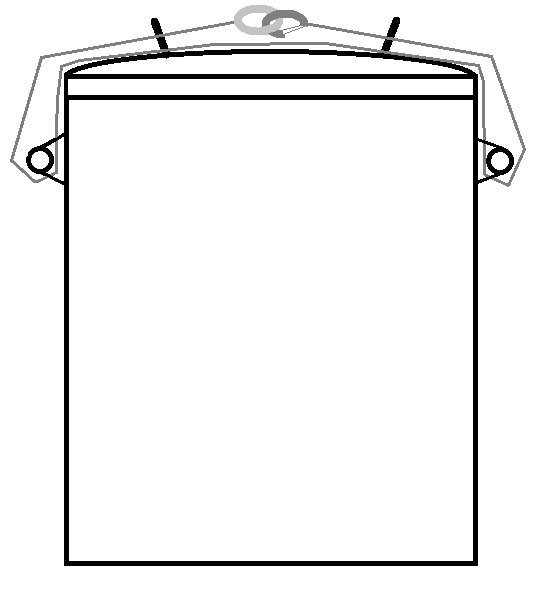
\includegraphics[height=8cm]{Cable.png} }}
    \caption{Securing the pressure vessel lid}
    \label{fig:sec_lid}
\end{figure}

        \end{itemize}    
    \item Pressurize the vessel
        \begin{itemize}
        \item \textbf{Safety glasses are required for everyone in the lab 
            anytime the vessel is pressurized}
        \item The absolute pressure in the vessel can be read at the bottom of 
            the TADA\_UI window
        \item Ensure the ball valve connecting the regulators to the inlet hose
            is closed (valve handle perpendicular to the flow)
        \item Fully open the rotometer on the exhaust of the pressure vessel by 
            \textbf{gently} rotating the rotometer knob counterclockwise 
        \item If it has not been done earlier in the day, slowly open the 
			cylinder valve all the way and then turn back one quarter turn
        \item Once the regulators are pressurized, slowly open the ball valve
        \item Slowly close the rotometer (rotate clockwise) until the air flow 
            reads 25 SCFH (The flow rate is read at the middle of the floating ball)
        \item Allow 1 - 2 minutes for equilibrium to be reached initially
        \item Adjust pressure in vessel using low pressure regulator until the    
            absolute pressure reading in the TADA\_UI is highlighted green 
            indicating that the pressure in the vessel is sufficiently close 
            to 1 atm (760 torr)
        
        \begin{itemize}
            \item This is easier with two people. One to read the pressure off 
                the TADA\_UI and the other adjust the regulator
            \item While pressurizing, make sure that the rotometer reads about 
                25 SCFH. This may take some adjusting back and forth.
            \item Ensure that there are no leaks around the lid before proceeding
			\item Allow at least 20 secs for equilibration each time the pressure 
				is changed
            \item \textbf{Leak protocol:} If a loud, high pitched noise is heard 
                or the pressure read on the TADA\_UI fails to rise, there is a 
                leak. If this occurs, do the following:
                \begin{itemize}
                \item Identify where the leak is happening (using the sound or
                    snoop A.K.A. Soapy water)
                \item If the leak is happening anywhere besides the O-ring,
                    immediately close the ball valve and allow the vessel to 
                    fully vent to ambient pressure to fix the leak
                \item If the leak is happening somewhere along the O-ring,
                    verify that there is no debris or wires breaking the seal.
                    If a seal break from debris or wires is found, immediately 
                    close the ball valve and allow the vessel to 
                    fully vent to ambient pressure to fix the leak
                \item If there is no debris or wires breaking the seal, use the
                    wrench to slowly tighten the clamp nuts around the leak 
                    until it stops
                \item If this does not work or you suspect a different problem,
                    immediately close the ball valve and allow the vessel to 
                    fully vent to ambient pressure to fix the leak
                \end{itemize}
            \end{itemize}
        \end{itemize} 

    \item Ensure the vessel is sufficiently dark to see any 
        flame from the mirror on top of the furnace
    
    \item In the TADA\_UI program, press the "Choose Target File" button and 
        choose where to save your file
        \begin{itemize}
        \item Save all temperature data files in comma separated values (.csv) 
            format
        \item Path: \textit{C:\textbackslash Users\textbackslash 
            Public\textbackslash Documents\textbackslash AIT\textbackslash 
            data\textbackslash compound\_name\textbackslash filename.csv}
        \item File naming convention: 
            \begin{itemize}
            \item Filenames will be organized by the following values in order 
                separated by underscores ("\_")
                    \begin{itemize}
                    \item Compound name
                    \item Date of experiment with the format "YYMMDD"
                    \item Time of day that data collection began for that run
                        using a 24 hour clock format "hhmm"
                    \item Sample size in microliters (for liquids) or milligrams
                        (for solids and gases)
                    \item Test temperature in degrees Celsius (rounded to the 
                        nearest integer)
                    \end{itemize}
                    
            \item For example: The file name of an AIT experiment where 100 
                microliters of hexane were tested at 450 \degree C on 
                March 19, 2013 at 4:25 pm would be: \newline
                "hexane\_130319\_1625\_100\_450.csv"
            \end{itemize}    
        \item This action will reset the TADA for measurement        
        \end{itemize}
    
    \item Begin data collection 
        \begin{itemize}
        \item In the TADA UI program, press the Enter key
        \item The TADA UI will keep track of the elapsed time since data 
          collection began at the bottom of the window. This may be used
          to time the experiment
        \end{itemize}
    
    \item Press the red button on the tablet screen to start recording
        
    \item Press the green or blue button on the ARIA control box that 
        corresponds to the physical state of the sample
        (green for solid, blue for liquid) to initiate ARIA sample injection.
        \begin{itemize}
        \item \textbf{NOTICE:} If you need to abort the injection before
            it completes, immediately unplug the AIRA power.
        \item If you mistakenly press the wrong button, do NOT abort the 
            injection. A button mis-press is inconsequential. Simply allow the 
            injection to complete then press the correct button.
        \end{itemize}
    
    \item Watch for an ignition event for 10 minutes
        \begin{itemize}
        \item Upon injection, a small temperature drop is always observed. This
            is the start of the 10 minutes
        \item A temperature rise above the initial temperature indicates an 
            exothermic reaction has occurred
        \item An ignition event is defined by the presence of a visible flame
            (visible to either the camera or the operator)
        \item An ignition event is characterized by a large, sharp temperature 
            rise exceeding $15 \frac{K}{s}$. This is referred to as
            a temperature spike
        \item The experiment ends when one of the following criteria is met:
            \begin{itemize} 
            \item An ignition event is observed and the temperature returns to 
                a steady state
            \item 10 minutes pass with no ignition event observed
            \end{itemize}
        \item Stop and power off the camera with the Capture app about 10 
            seconds after a temperature spike occurs or after a visible flame 
            disappears
        \item If temperature spike is observed, allow enough time for the
            temperature to return to a steady state before terminating 
            temperature data collection
		\item If no ignition event is observed nor expected, after a 
            temperature rise reaches a maximum the camera may be stopped 
            before 10 minutes have elapsed
        \item The TADA\_UI may be used to keep track of time
        \end{itemize}
    
    \item If necessary, review the camera footage, looking for a flame 
        corresponding to the temperature spike
        \begin{itemize}
        \item This may be done on the Capture app on the tablet
        \end{itemize}
    
    \item Record pertinent data and observations in the lab book and 
        the TADA\_UI \textbf{BEFORE} terminating temperature data collection
        \begin{itemize}
        \item The following data must be present on the same row in the lab 
            notebook, in the following order:
            \begin{itemize}
            \item Time of day that data collection began
            \item Compound name 
            \item Sample size in microliters (for liquids) or milligrams
                (for solids and gases)
            \item Set-point temperature of the furnace
            \item Test temperature in degrees Celsius (rounded to the 
                nearest integer)
                \begin{itemize}
                \item This should be the internal flask temperature 
                    (Thermocouple 4) prior to injection
                \end{itemize}
            \item Indicate the type event that took place ("h" for hot-flame 
                ignition, "c" for cool-flame ignition and "n" for no ignition)
                \begin{itemize}
                \item If the flame is bright yellow/orange, this is considered a 
                    hot-flame autoignition
                \item If the flame is faint and blueish, this is considered a 
                    cool-flame autoignition
                \end{itemize}
            \item Indicate if any sound was heard upon ignition (if applicable)
            \end{itemize}
       
        \item If any item is not applicable write down N/A in its place
        \item If any item is unknown, leave it blank until it can be determined
        \item Optionally, leave any pertinent comments about the experiment
            next to or directly under this row of data
        \item Record the same data in the corresponding fields in the TADA UI
            \textbf{before} terminating temperature data collection
        \item The lot number and/or sample number of the container with the 
            supplier and any other pertinent information related to the source
            of the compound should be recorded at least once in the lab 
            notebook. Ensure that these data are present
        \end{itemize}
        
    \item After the experiment ends, terminate data collection
        \begin{itemize}
        \item Press the Enter key  again to stop data 
            collection (the red light on the TADA should stop blinking)
        \item If you haven't already, press the red button on the tablet screen 
        to stop recording
        \item Shut down the camera from the tablet
        \end{itemize}
        
    \item Set furnace to next temperature

    \item Wait about 20 minutes after ignition to allow for the pressure 
        vessel to be purged of the combustion products. If there was no ignition,
		only wait 10 minutes for the pressure vessel to purge after the experiment ends 
    \item After the purge time has ended, depressurize the vessel
        \begin{itemize}
        \item Turn off the inlet air flow using the ball valve
        \item Fully open the rotometer by gently turning the knob counterclockwise
		\item Wait until the pressure vessel is \textbf{fully} depressurized (i.e. the rotometer 
            reads zero)
        \end{itemize}
    \item Remove the pressure vessel lid by \textbf{first} loosening and 
        disengaging the clamps and \textbf{secondly} removing the safety cable
        \begin{itemize}
        \item Loosen the clamps using a 3/4" wrench instead of a 
            torque wrench
		\item Break the seal on the lid by briefly lifting the lid with the safety cable still in 
                place
        \item Remove the safety cable from the vessel
        \end{itemize}
    \item \textbf{Simultaneously} Lift off the lid and place snorkel inside the pressure vessel 
        between 6" and 10" over the furnace
        \begin{itemize}
        \item Two people should perform this step. One to remove the lid and one
            replace the snorkel inside the vessel
        \end{itemize}
	\item Remove the camera from the vessel
    \item Remove any syringe or weigh boats used in the previous experiment
        \begin{itemize}
        \item \textbf{Use gloves when doing this}
        \item Dispose of any weigh boats in the solid waste
        \end{itemize}
    \item Clean out the flask between measurements by blowing hot air into
            the flask for 5 minutes using the heat gun on the low setting
        \begin{itemize}
        \item The heat gun should \textbf{only} be plugged in to the outlet 
            when in use
        \item Do not point the heat gun towards the ARIA at any time
        \end{itemize}
    
    \item Extract, save and appropriately rename the video data between experiments    
    \item Once the next temperature is reached, allow the system to come to 
        equilibrium
        \begin{itemize}
        \item The "Temp Ready" indicator in the TADA\_UI window should turn 
            green when the system has come to an acceptable equilibrated state
        \item Once the system is at equilibrium, begin experiments
        \end{itemize}
    \item Once the system is at equilibrium, start this procedure over from 
        step 1 (Measure Out Sample)
    \end{enumerate}

    
\subsection{Shutdown}
    \begin{itemize}
    \item The following should be done before leaving the lab at the end of 
        every work day or any time the setup is not in use:
        \begin{enumerate}
        \item Power off the furnace
        \item Close the TADA\_UI program
        \item Unplug TADA USB connection
        \item Unplug the wall power from the TADA power supply
        \item Unplug the ARIA power supply cable
        \item Shut down and unplug the tablet
        \item Turn the camera Wi-Fi off then shut down and unplug the camera
        \item Extract all data to the computer and appropriately rename them 
            (Refer to Section \ref{sec:data})
        \item Close all programs and shut down the computer
        
        \item Remove and store any ARIA accessories used that day (leave the 
            ring stand in place)
        \item Clean the funnel with appropriate solvents and dispose of the waste
        \item Discard the contents of both beakers and prepare them for dish washing
        \item Discard any residual sample in syringes and store them in the syringe box in the AIT
            drawer without rinsing %% Change POLICY for syringes
        \item Store all chemicals in the appropriate cabinets
        \item Remove any organic solid residue from working surfaces 
            (See Section \ref{sec:spill_solid})
		
		\item Ensure all air systems are depressurized 
			\begin{itemize}
			\item Ensure the ball valve is closed (the handle should be perpendicular to the flow)
			\item Slowly close the cylinder valve all the way
			\item Open the ball valve by turning the handle parallel to the flow
            \item Wait until both regulators depressurize
			\end{itemize}
        \end{enumerate}
    
    \item A hot furnace may be left with the pressure vessel open and the snorkel 
        venting it without waiting for it to cool
    \item Under normal use, disposable gloves may be thrown into the normal 
        trash receptacle instead of solid chemical waste
    \end{itemize}

\newpage    

\section{Data Extraction} \label{sec:data}
During experiments data are being recorded on the lab computer, the data logger 
and the camera. Both the camera and the data logger on the TADA have SD cards 
with a 32 GB storage capacity that allows multiple runs to be recorded without 
extraction. The following policies are in place to ensure ease of use, 
efficiency and avoid common mistakes.
    \begin{itemize} 
    \item For the AIT setup, do not exceed 10 runs without extracting 
        temperature data to the computer and deleting the data from the SD  
        cards.
    \item All data should be extracted at least \textit{daily}
    \item Video data should be extracted and properly renamed as often as  
        possible (i.e. between every run or every other run) to ensure the 
        correct filenames are assigned to their corresponding video files
    
    \item File naming convention: 
        \begin{itemize}
        \item Filenames will be organized by the following values in order 
            separated by underscores ("\_")
                \begin{itemize}
                \item Compound name
                \item Phase of the compound ('g' for gases, 'l' for liquids,
                    's' for solids)
                \item Date of experiment with the format "YYMMDD"
                \item Time of day that data collection began for that run
                    using a 24 hour clock format "hhmm"
                \item Sample size in microliters (for liquids) or milligrams
                    (for solids and gases)
                \item Test temperature in degrees Celsius (rounded to the 
                    nearest integer)
                \end{itemize}
                
        \item For example: The filename for temperatures from an AIT experiment  
            where 100 microliters of liquid hexane were tested at 450
             \degree C on March 19, 2013 at 4:25 pm would be: \newline 
            "hexane\_l\_130319\_1625\_100\_450.csv"
        \end{itemize}

    \item Video and data logger data must be processed (i.e. parsed, edited, 
        timestamped etc.) before being organized and therefore will be saved to 
        the same path initially

    \item After processing, all data should be organized according to the 
        following path convention:
        \begin{itemize}
        \item Path: \textit{C:\textbackslash Users\textbackslash 
            Public\textbackslash Documents\textbackslash AIT\textbackslash 
            data\textbackslash compound\_name\textbackslash filename.ext}
        \item All data, including videos, from the same run should have the same
            filename and path but different extensions except data from the 
            datalogger
        \item The datalogger filename convention should also have '\_dlog' at 
            the end of the name to distinguish it from the UI generated file 
            (e.g. "hexane\_l\_130319\_1625\_100\_450\_dlog.csv")
        \item When processing is finished all runs should have the following 
            4 files with the same name preceding them
            \begin{itemize}
            \item A .xlsx file (for temperature data with graphs and analysis)
            \item A .csv file (UI generated)
            \item A \_dlog.csv file (datalogger)
            \item A .avi/.mp4 file (video)
            \end{itemize}
        \end{itemize}

    \item The camera may be plugged in via USB and video extracted with
        GoPro\textsuperscript{\textcopyright} Quik software
        \begin{itemize}
        \item Connect the camera to the computer via a micro USB cable (See 
            Figure \ref{fig:cam_diag})
        \item Press the "info/wireless" button on the camera to connect the 
            camera to the computer
        \item Quik should be configured to open automatically extract video 
            when the camera connects to the computer
        \item Video files should be extracted to the DIPPR legacy server and 
            organized by date:
            \begin{itemize}
            \item Path: \textit{\textbackslash \textbackslash 
               dipprlegacy.et.byu.edu\textbackslash aitra\textbackslash 
               video\_import}
            \item Username: dipprleg\textbackslash aitra
            \item Password: hotflame16
            \end{itemize}
        \item If Quik is not configured to do this refer to the Quik manual for
            how to configure this (or ask me and I will configure it)
            \begin{itemize}
            \item \textit{C:\textbackslash Users\textbackslash 
            Public\textbackslash Documents\textbackslash AIT\textbackslash 
            docs\textbackslash GoPro\_App\_for\_Desktop\_User\_Manual.pdf}
            \end{itemize}
        \item Once extracted to the DIPPR legacy server, video data may be 
            timestamped and converted to .avi format on the server
        \end{itemize}
        
    \item To extract data from the data logger
        \begin{itemize}
        \item Unplug the TADA from the computer
        \item Pull out the SD card from the data logger and use the USB SD card 
            adapter to copy the"DATALOG.CSV" file into the "raw\_data" path and 
            rename it to the original filename with the date 
            tagged on in "YYMMMDD" format (e.g. "DATALOG\_130319.CSV")
            \begin{itemize}
            \item Path: \textit{C:\textbackslash Users\textbackslash 
            Public\textbackslash Documents\textbackslash AIT\textbackslash 
            data\textbackslash raw\_data}
            \end{itemize}
        \item Open the "DATALOG.CSV" file on the SD card, erase all data from
            it and save it, making sure to not change its name, extension or 
            file path
        \item Close all windows with the USB SD card adapter open (i.e. Excel 
            files, Windows Explorer etc.)
        \item Pull out the SD card without ejecting the unit from the computer
        \end{itemize}
    
    \item Ensure all files from the camera and data logger are deleted after they
        have been properly saved in the data folder 
            
    \end{itemize}
    
\newpage
\section{Spill Clean-up}
In the event of any spill, appropriate PPE specified in the corresponding SDS 
    should be used in clean-up. Always check the SDS for special considerations
    when cleaning up any compound.
    \subsection{Liquids}
    \begin{itemize}
    
    \item In the event of a small spill (i.e. less than 100 ml), the following 
        protocol should be followed:
        \begin{itemize}
        \item If the spill occurs in or out of the hood, use absorbent clay that
            can be found under the counter west of the sink to soak up the 
            bulk of the liquid and wipe up the rest with a paper towel
        \item Dispose of the clay, any disposable gloves and towels in the solid 
            waste container
        \end{itemize}    
    \item In the event of a large spill (i.e. greater than 100 ml), the 
        following protocol should be followed:
        \begin{itemize}
        \item If the spill occurs in the hood, use absorbent clay that can be 
            found under the counter on the left-hand side of the lab sink to 
            soak up the bulk of the liquid and wipe up the rest with a paper 
            towel
        \item Dispose of the clay, any disposable gloves and towels in the solid 
            waste container
        \item If the spill occurs outside the hood or the spill is particularly 
            large (e.g. an entire bottle of a flammable material breaks) 
            \textbf{perform the Emergency Shutdown Procedure (Section 
            \ref{sec:e_shtdn}), evacuate the lab and call: BYU Risk Management 
            and Safety - (801)-422-4468} 
        \end{itemize}
    
    \item Spills involving compounds that are particularly toxic or unstable 
        should always be considered large spills
    
    \end{itemize}

    \subsection{Solids} \label{sec:spill_solid}
    We will generally work with organic solids that readily dissolve in simple
    organic solvents (e.g. acetone). Researchers must always check chemical 
    compatibility with solutes and solvents before dissolving any compound.
    \begin{itemize}
    \item Small amounts of organic solids may be dissolved in a small amount of 
        solvent and put in organic liquid waste
    \item Larger amounts of solids should be transferred to solid waste and the
        residue should be dissolved in solvent and discarded in liquid waste
    \end{itemize}

\newpage    
\section{Emergency Shutdown} \label{sec:e_shtdn}

    \begin{itemize}
    \item In the event of an emergency do the following:
        
        \begin{itemize}
        \item Close the air cylinder valve
        \item Power off and unplug the furnace
        \item Fully open the rotometer exhaust
        \item Unplug all other electrical equipment
        \item Stop the camera recording (if applicable)
        \item Shutdown and unplug the camera and tablet
        \item Close all programs and shutdown the computer
        \end{itemize}
    
    \item If an emergency requires you to evacuate the lab, do only the first 
        2 steps
    \item \textbf{DO NOT perform any steps that present a danger to you}
    \end{itemize}

\newpage
\section{Experimental Setup and Maintenance}
    \subsection{Furnace}
        \subsubsection{Overview}
    \begin{itemize}
    \item The furnace, shown in Figure \ref{fig:furnace_pic}, is an encased 
        stack of ceramic insulation with cavities 
        cut out to allow space for the heating elements and the test flask
        (see Figure \ref{fig:in_furnace} for an internal diagram of the 
        furnace). The furnace is controlled with measurements taken at the 
        insulated furnace wall. This design causes the furnace to have
        large temperature gradients while in operation. As a result, the 
        set point temperature and the flask temperature will almost always 
        differ significantly (as much as 25 K in some cases). Therefore, 
        set points must be chosen between approximately 10 - 20 K above the 
        desired temperature to reach that temperature inside the flask.
        \textbf{The reported AIT must be taken from the internal flask 
        temperature (Thermocouple 4) and NOT the control thermocouple inside
        the furnace}
    
    \begin{figure}[H]
    \centering
    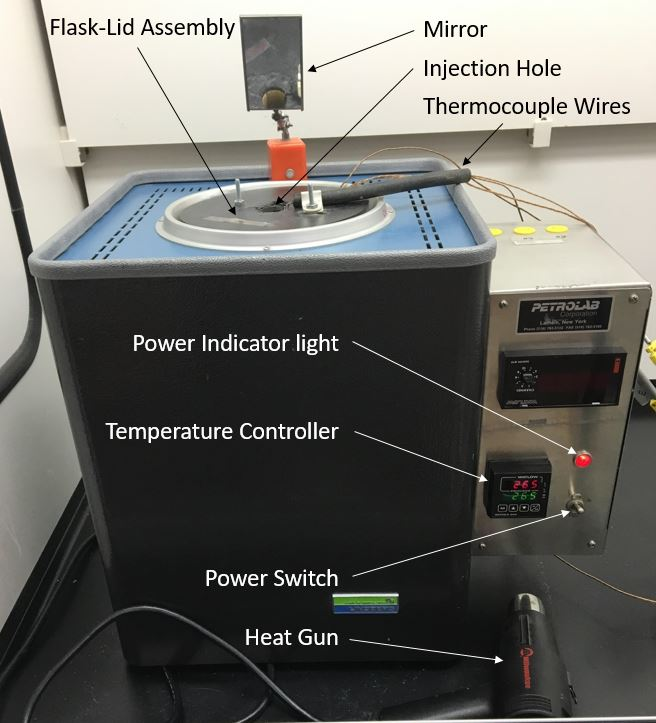
\includegraphics[width=.45\textwidth]{Furnace_pic_diagram.jpg}
    \caption{AIT Furnace}
    \label{fig:furnace_pic}
    \end{figure}
    
    \item When powered on initially, the furnace may take up to 2 hours or more  
        to reach a desired temperature and thermally equilibrate
    \item Any time a desired temperature is reached, allow at least 30 
        minutes for thorough thermal equilibration in the flask; allow extra 
        time during initial start up
     
     \end{itemize}

\subsubsection{Furnace Operation}
See Figure \ref{fig:furnace_pic} for reference on how to operate the furnace
      \begin{itemize}
      \item Power on the furnace with the power switch and use the temperature
            controller to choose a set point temperature
        \begin{itemize}
            \item To change the set point, press the up or down     arrows until 
                the desired temperature is reached
            \item The lower (green) display is the set point and     the upper 
                (red) display is the control thermocouple temperature
        \end{itemize}
        
        \item When shutting down, turn off the power switch and unplug the furnace
        \end{itemize}

        
    \subsection{Camera and Tablet} \label{sec:cam_tab}
    \subsubsection{Overview}
        \begin{itemize}
        \item Prior to using the experimental setup, all researchers must become 
        familiar with basic use and operation of the 
        GoPro\textsuperscript{\textcopyright} HERO4
        Session\textsuperscript{TM} camera and the Samsung Galaxy Tab A Tablet. 
        
        More detailed instructions on how to do basic tasks may be found at the 
        following URLs:
        \begin{itemize}
        \item \texttt{https://shop.gopro.com/softwareandapp}
        \item \texttt{https://gopro.com/help/articles/Block/How-to-Pair-the-Camera-with-the-GoPro-App\#HERO4 Session}
        \item \texttt{https://gopro.com/help/articles/Block/Getting-Started-with-the-GoPro-App}
        \item \texttt{http://www.samsung.com/us/support/owners/product/galaxy-tab-a-8-0-wi-fi}
        \end{itemize}
    
    
\begin{figure}[H]
\centering
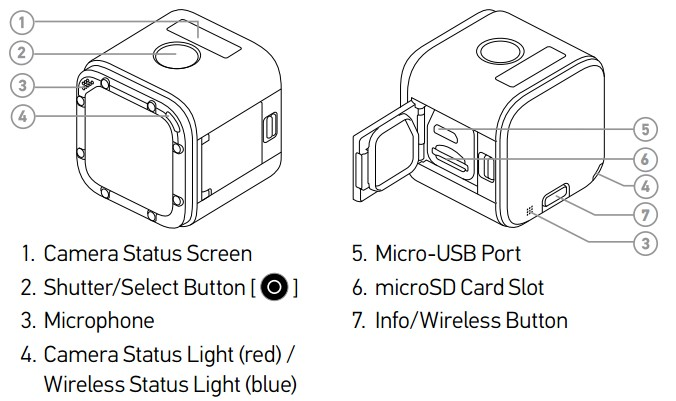
\includegraphics[width=.6\textwidth]{Camera_diagram.jpg}
\caption{GoPro\textsuperscript{\textcopyright} HERO4
        Session\textsuperscript{TM} Camera Parts}
\label{fig:cam_diag}
\end{figure}

\begin{figure}[H]
\centering
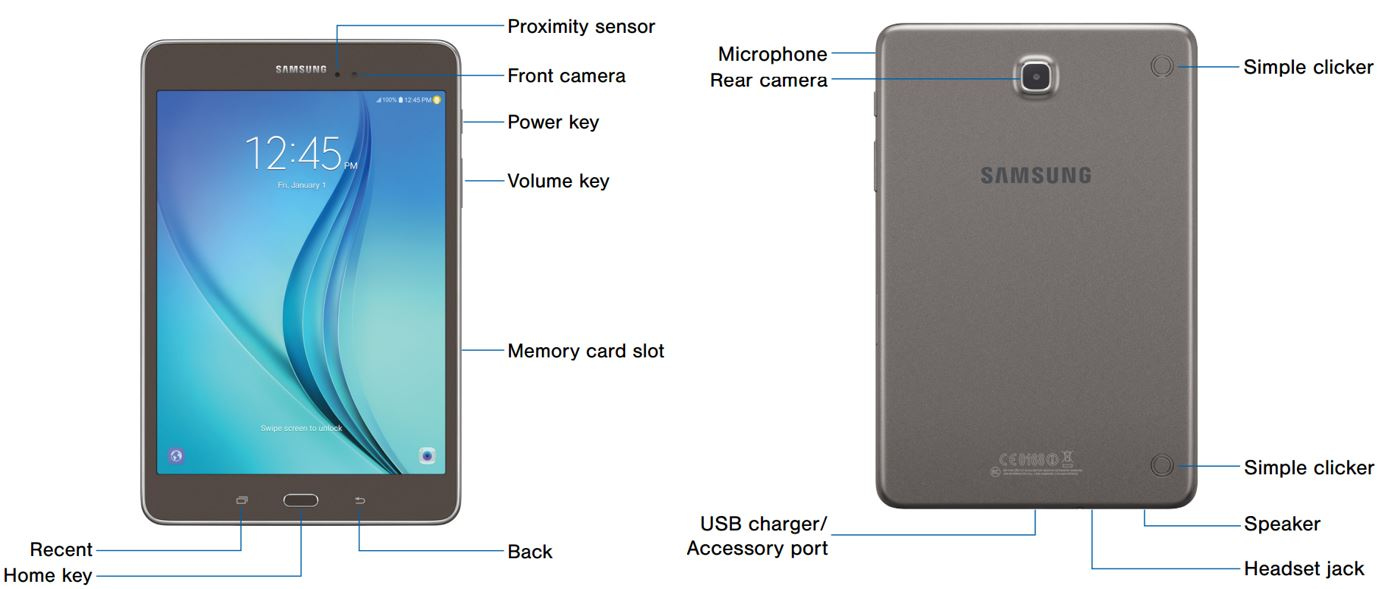
\includegraphics[width=1\textwidth]{tablet.jpg}
\caption{Samsung Galaxy Tab A}
\label{fig:tablet}
\end{figure}
    
    \item Refer to Figures \ref{fig:cam_diag} and \ref{fig:tablet} for camera 
        and tablet setup
        
     \end{itemize}
        
       
    \subsubsection{Connecting to the camera} 
        \begin{itemize}
        \item Firmly press and release the ``info/wireless" button on the back of
            the camera (not the red circle) multiple times until you see \
            ``APP \& RC" on the camera status screen
        \item Press the ``shutter/select" button (the button with the red 
            circle) to confirm your selection
            \begin{itemize}
            \item The ``wireless status" (blue) light will begin flashing. This 
                indicates the camera is broadcasting a Wi-Fi signal 
            \end{itemize}
        \item Power on the tablet by holding down the power key (top, right side) until you see the
            splash screen indicating the tablet is booting up
        \item When first powering on both devices ensure they both are 
            sufficiently charged. If not, immediately plug them in
        \item Once the tablet has booted, swipe to get to the home screen and 
            select the ``Settings" app
        \item Select the Wi-Fi settings at the top of the list on the left side 
            of the screen
        \item Select the Wi-Fi network labeled ``ait\_cam\_2016" then select 
            ``connect" on the message box that pops up (FYI: the wifi password is
            ``hotflame16")
        \item Once the tablet has connected to the Wi-Fi, return to the home 
            screen by pressing the home key
        \item Open the GoPro Capture App (app is labeled ``Capture" on the home 
            screen) 
        \item Select the connect box on the top left corner of the screen to connect to camera
        \item Press the camera icon in the center of the screen
            \begin{itemize}
            \item The camera will make a beeping noise and the camera view will 
                open on the tablet
            \end{itemize}
        \end{itemize}
    
    \subsubsection{Shutdown}
        \begin{itemize}
        \item To shutdown the camera:
            \begin{itemize}
            \item Press the ``info/wireless" button 
                until the camera status screen reads ``Turn Wi-Fi Off"
            \item Press the ``shutter/select" button to confirm your selection
                \begin{itemize}
                \item The ``wireless status" (blue) light will stop flashing
                \end{itemize}
            
            \item Press the ``info/wireless" button until the camera status 
                screen reads ``Exit"
            \item Press the ``shutter/select" button to confirm your selection
                \begin{itemize}
                \item The camera will shutdown 
                \end{itemize}
            
            \end{itemize}
        
        \item To shutdown the tablet:
            \begin{itemize}
            \item Press the ``Recent" button to bring up all opened programs and 
                close all programs by swiping on them or pressing the 'X' in the
                top right corner
            \item Press and hold the Power key until the option to power of 
                pops up then press power off
                \begin{itemize}
                \item The tablet will shutdown
                \end{itemize}
           
            \end{itemize}
        
        \end{itemize}
    
    \subsubsection(Camera Placement and Removal)  \label{sec:cam_on_furn}
        \begin{itemize}
        \item To mount the camera on the furnace:
            \begin{itemize}
            \item Lift the rubber flap on the base of the camera buckle 
                out of the way to allow the buckle to slide into the camera 
                mount 
            \item Insert the plastic buckle into the camera mount on the side 
                of the furnace until it snaps securely into place
            \item Press the rubber flap back into place to lock the camera 
                buckle into the camera mount 
            \end{itemize}
        \item To remove the camera from the furnace:
            \begin{itemize}
            \item Lift the rubber flap on the base of the camera buckle 
                out of the way to allow the buckle to slide out of the camera 
                mount
            \item Squeeze the two catches on the camera buckle and pull the 
                buckle out of the camera mount
            \end{itemize}
        \end{itemize}
    
    \subsubsection{Other Information}
        \begin{itemize}
        \item Camera Operation
            \begin{itemize}
            \item All operations may be done remotely on the tablet via Wi-Fi or 
            directly with the ``info/wireless" and ``shutter/select" buttons on 
            the camera. For experimental purposes, only basic operations
            will be covered. For more detail on camera 
            operation please see the URLs above
            \item In the camera's off or normal modes the ``shutter/select" button 
            toggles recording or standby; the camera will automatically shut off
            after a few seconds on standby
            \item If the camera is remotely controlled, the on screen red button 
            toggles recording or standby
            \item During recording, the camera will not allow viewing via the 
            tablet. This is due to the high frame rate of our experiments
            \item Captured video may be reviewed and managed remotely with the grid
            button on the bottom left corner of the screen
            \item The camera may be powered on and off remotely with the power  
            button on the top right corner of the screen. The camera should be 
            powered off between experiments or when not in use
            \end{itemize}
        
        
        
        \item Batteries:
            \begin{itemize}
            \item Recharging power supplies and USB cables are available for both
            the tablet and camera
            \item Both the camera and the tablet may be charged while in use
            \item Do NOT charge tablet with the computer as it does not deliver 
            enough current for effective charging
            \item Batteries should be allowed to discharge to between 10 - 20\%
            before recharging
            \item Batteries should always be recharged to 100\% capacity before 
            unplugging
            \item Do not overcharge any battery. Do not leave any battery 
            charging overnight
            \end{itemize}
        
        \end{itemize}

\subsection{Pressure Vessel}
\subsubsection{Changing the rupture disk}
We use 1100 alloy extra thin aluminum foil as a rupture disk. This material has 
been shown to be effective in preventing catastrophic failure in the vessel. 
These sections outline how to change and test the rupture disk. (See Figures 
\ref{fig:rupture disk_assemble} and \ref{fig:rupture_disk} for reference)

\begin{figure}[H]
    \centering
    \subfloat[O-ring on Foil]{{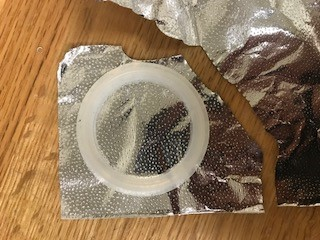
\includegraphics[height=4cm]{o_ring_on_foil.jpg} }}
    %\qquad
    \subfloat[Sandwich the foil between O-ring and TC outlet 
        ring]{{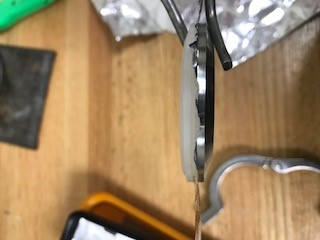
\includegraphics[height=4cm]{cap_and_o_ring.jpg} }}
    \subfloat[Fold the foil back] {{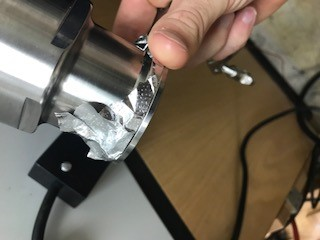
\includegraphics[height=4cm]{fold_foil.jpg} }}
    \caption{Installing a new rupture disk}
    \label{fig:rupture disk_assemble}
\end{figure}

    \begin{enumerate}
    \item Remove the O-ring and the TC outlet ring from the pressure vessel by 
        removing the TC clamp (See Figure \ref{fig:rupture_disk})
    \item place the O-ring on a piece of extra thin 1100 alloy aluminum foil
        \begin{itemize}
        \item \textbf{Do NOT use the aluminum foil used for wrapping the flask,
            it is far too strong and may lead to a catastrophic failure of the 
            vessel}
        \end{itemize}
    \item Rip the foil around the O-ring so it roughly matches the area of 
        the O-ring
    \item Sandwich the ripped foil in between the O-ring and the outlet ring
    \item Place the combined rings and foil on the rupture outlet on the 
        pressure vessel and fold any excess foil over the rupture outlet on the 
        pressure vessel 
    \item Secure the assembly on the pressure vessel using the TC clamp
        \begin{itemize}
        \item The foil should appear smooth across the rupture surface without any 
            folds or crumpled spots
        \item The studded surface may still be apparent; this is normal
        \end{itemize}
    \end{enumerate}

% \subsubsection{Testing the rupture disk}
    % \begin{itemize}
    % \item Securely attach the rupture disk testing device to the low pressure
        % regulator
    % \item Put on safety glasses and use earplugs
    % \item Take the O-ring and place it on a piece of tin foil
    % \item Using your fingers, rip the tin foil around the O-ring
    % \item Take the piece of tin foil and place it in between the O-ring and the cap
    % \item Fold the excess tin foil over so that it is not in the way
    % \item Secure the cap on using the clamp
    % \item Open the air tank by screwing the cap counterclockwise
    % \item Slowly turn the pressure regulator clockwise so and observe the increase in pressure (PSI)
    % \item Observe at what pressure the tin foil failed
    % \item Turn the pressure regulator counterclockwise to decrease the pressure
    % \item Unplug the pressure regulator
    % \item Close the air Tank by screwing the cap clockwise
    % \item Record the Pressure at which it failed, whether the shiny or dull 
        % side was facing outwards, if the foil was original smooth or crumpled, 
        % and where the hole appeared
    % \end{itemize}

\newpage
\subsection{Flask and Lid}
    \begin{itemize}
    \item \textbf{Latex or nitrile gloves and safety glasses are 
            required while working with the flask/lid assembly}
    
    \item Using the TADA\_UI, check the temperature of the furnace to ensure 
        safe handling before changing the flask
        \begin{itemize}
        \item The temperature should be close to ambient lab temperature
        \item Do not perform maintenance or change the flask unless the 
            internal temperature of the furnace is below $40^\circ C$
        \end{itemize}
    
    \item The flask in the furnace must be exchanged for a clean flask in the 
        following situations:
        \begin{itemize}
        \item The next experiment will be for a different compound
        \item The next experiment will be for a new container of the same 
            compound
        \item There is reason to suspect that the flask has become 
            contaminated or substantially dirty
        \item The flask has been used for 10 runs without being cleaned
        \item Once the AIT has been found for a compound, the final measurements
            should be repeated with a clean flask to verify the results
        \end{itemize}
    
    \item Disassembling the Flask and Lid
        \begin{itemize}
        \item \textbf{The furnace may be too hot to open for several hours after
             an experiment}
        \item Unplug the thermocouples from the furnace
        \item Once the furnace is cool, remove flask/lid assembly
            \begin{itemize}
            \item Loosen (do NOT remove) the nut that secures the bracket and 
                the rubber hose to the top of the furnace with a wrench
            \item Move the bracket out of the way and remove Thermocouple 4 
                (along with the rubber hose) from the top of the furnace
            \item Move the mirror out of the way to allow the flask/lid assembly
                to come out. Likewise ensure that the ARIA is out of the way
            \item Grip the assembly with both hands by the screws on top and 
                pull directly upward
            \item \textbf{NOTE: The flask/lid assembly is heavy and pulling it  
                out can be awkward. Please ask someone to help you remove it 
                if you are at all unsure about removing the assembly}
            \item The flask/lid assembly should easily come out of the furnace 
                without catching on anything
            \end{itemize}
        
        \item \textbf{Carefully} set the assembly on a table or other stable 
            surface with the flask on top (See Figure \ref{fig:f_lid_done})
        \item Ensure the bracket screw is loose
        \item Remove the circular spring from its groove and slide the ceramic
            halves of the lid apart sufficiently to allow the flask to be 
            removed
        \item Remove flask from lid assembly and  remove all of the aluminum 
            foil and thermocouples from the flask
        \item Discard the used aluminum foil in a normal trash can and set 
            aside the thermocouples in the hood or on a surface where they will
            not catch on anything or become damaged
        \item \textbf{Always store bulb flasks on the drying rack above the sink 
            or appropriately secured to a ring stand} (see "Flask Cleaning"
             section)
        \end{itemize}

\newpage      
    \item Assembling the Flask and Lid 
        \begin{itemize}
        \item Use the figures in this section as a reference when putting 
            together the assembly
        
        \item Use a \textbf{clean}, 500 ml, round bottom, long neck, bulb flask 
            (PYREX\textsuperscript{\textcopyright} 500mL Long Neck Boiling 
            Flask, Round Bottom, Tooled Mouth, Product No.: 4280-500 from 
            Corning Inc.)
        \item If dirty, wash out the flask using soap and water and dry as much 
            as possible (see ``Flask Cleaning" section); be sure to rinse
            thoroughly
                \begin{itemize}
                \item Any leftover water will boil away when the furnace heats 
                up and before any measurements are taken
                \end{itemize}        
        \item Wrap entire flask in aluminum foil with thermocouples at the 
            bottom, side and top of the round part of the flask (thermocouples 
            should be touching the glass directly) (Refer to Figure 
            \ref{fig:wrap})
                \begin{itemize}
                \item NOTE: The more reflective side of the foil should always 
                    be facing inward
                \item Start by getting a long strip of aluminum foil (12" long 
                    or so)
                \item Use a utility knife to poke a small hole (just big enough 
                    to poke the bead through) near the middle of 
                    the foil and insert thermocouple 3 through the foil so the 
                    bead sits at the bottom of the flask and then wrap the foil 
                    around the bottom (1 and 2)
                \item Slide thermocouple 2 down to the approximate 
                    middle/equator of the flask between the flask and foil and run
                    a couple of inches around the equator so that it stays in place  
                \item Use a second piece of foil to wrap further up the flask, 
                    ensuring the thermocouple wires run parallel up the side of 
                    the flask (3)
                \item Place thermocouple 1 at the top of the bulb of the flask 
                    (not on the neck of the flask) and use a third piece of foil
                     to wrap around the top starting at the middle (4)
                \item Add an additional layer of foil around  the flask so the 
                    wires are covered and run parallel when wrapping is finished
                    (5)
                \item Wrap additional foil around the neck of the flask to cover 
                    it completely and secure flask in lid assembly
                \item The thermocouple wires should emerge from the foil 
                    covering near the top (but not at the top) of the flask 
                    neck, allowing them to run between the two ceramic halves of
                    the lid assembly (6)
                \end{itemize}

\begin{figure}[H]
\centering
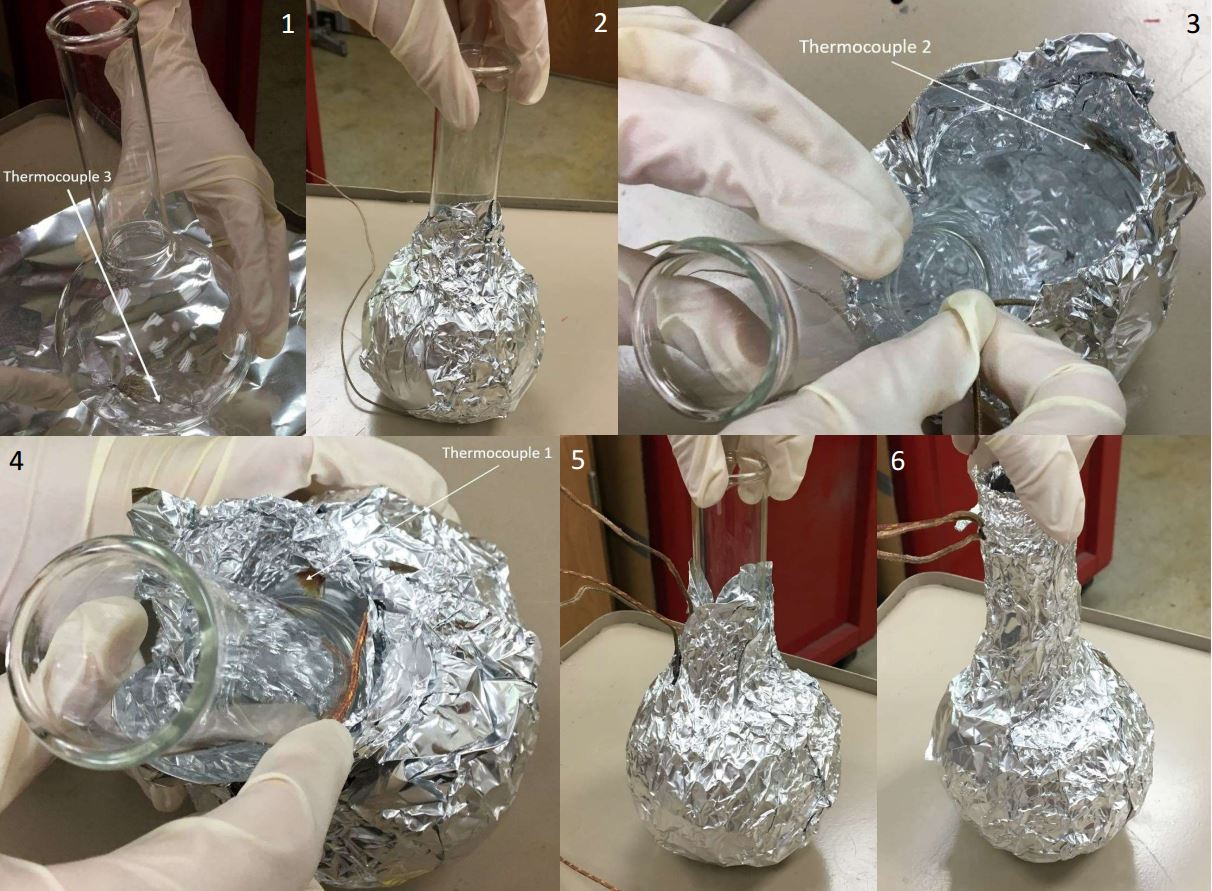
\includegraphics[width=1\textwidth]{wrap.jpg}
\caption{Steps for wrapping the flask in foil}
\label{fig:wrap}
\end{figure}

        \item Ensure the bracket screw is loose
        \item Fit the neck of the flask in the center hole of the ceramic lid 
            assembly with the lip of the flask fitting into the groove at the 
            base of the center hole on both sides
        \item Guide the thermocouple wires in the gap between the two ceramic 
            halves so they are out of the way when the flask/lid assembly is 
            inserted into the furnace
        \item Slide the loose half of the ceramic back in to be snug 
            around the flask neck, replace the spring, and tighten the nut on the top to hold it
            in position
                \begin{itemize}
                \item The two halves nearest to the top of the assembly should 
                    meet or very nearly meet; if they don't then some 
                    foil should be removed from the neck of the flask
                 \end{itemize}
        \item Use a circular spring to help hold the halves together
               
        
        \item Make a ``donut" of foil wrapped around the neck of the flask that 
            will rest up against the bottom of the lid assembly
        \item Slide the foil ``donut" up so and press it so it is flush against 
            the ceramic and restricts air flow around the opening
        \item Carefully turn the flask/lid assembly over making sure the flask 
            doesn't fall out
                \begin{itemize}
                \item \textbf{Do this over a table or close to a level surface 
                    to avoid accidental breaking of the flask}
                \item The flask will fit into the lid assembly somewhat loosely, 
                    but it shouldn't fall out
                \item If the flask falls out, remove it and add more foil 
                around the neck
                \end{itemize}
         
\begin{figure}[H]
\centering
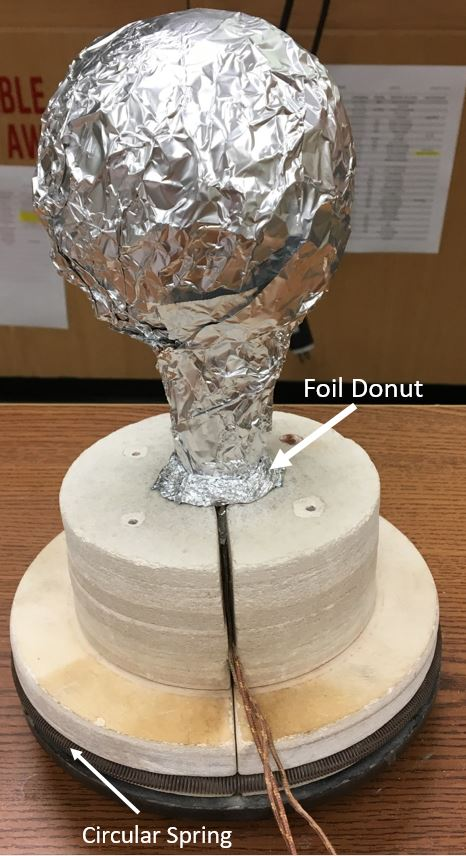
\includegraphics[width=.45\textwidth]{insert_in_lid_w_donut.jpg}
\caption{Final state of the flask/lid assembly}
\label{fig:f_lid_done}
\end{figure}
        
        \item See Figure \ref{fig:f_lid_done} for the final flask/lid
            assembly before insertion into the furnace
        \item Place the prepared flask/lid assembly into the furnace by gripping
            the assembly with both hands by the screws on top and slowly 
            lowering the assembly into place
        \item Turn the flask/lid assembly so the thermocouple wires point away 
            from the ARIA
        \item Insert flask interior thermocouple (\#4) carefully down the flask 
            neck, making sure it goes straight in and the bead doesn't get 
            caught anywhere
                \begin{itemize}
                \item The bead of Thermocouple 4 should be suspended in the 
                    approximate center of the flask, not be touching any part
                \item The wire of Thermocouple 4 should run up the edge of the 
                    neck and not the middle to allow compound to be injected 
                    without making contact with the thermocouple
                \item Use the bracket on one of the two screws on top of the 
                    lid to secure the rubber hose holding the thermocouple
                    in place
                \item Tighten the nut on the bracket hand tight and then give a 
                    half turn with a wrench to secure the nut (See Figure 
                    \ref{fig:wrench_tight})
                \end{itemize}

\begin{figure}[H]
\centering
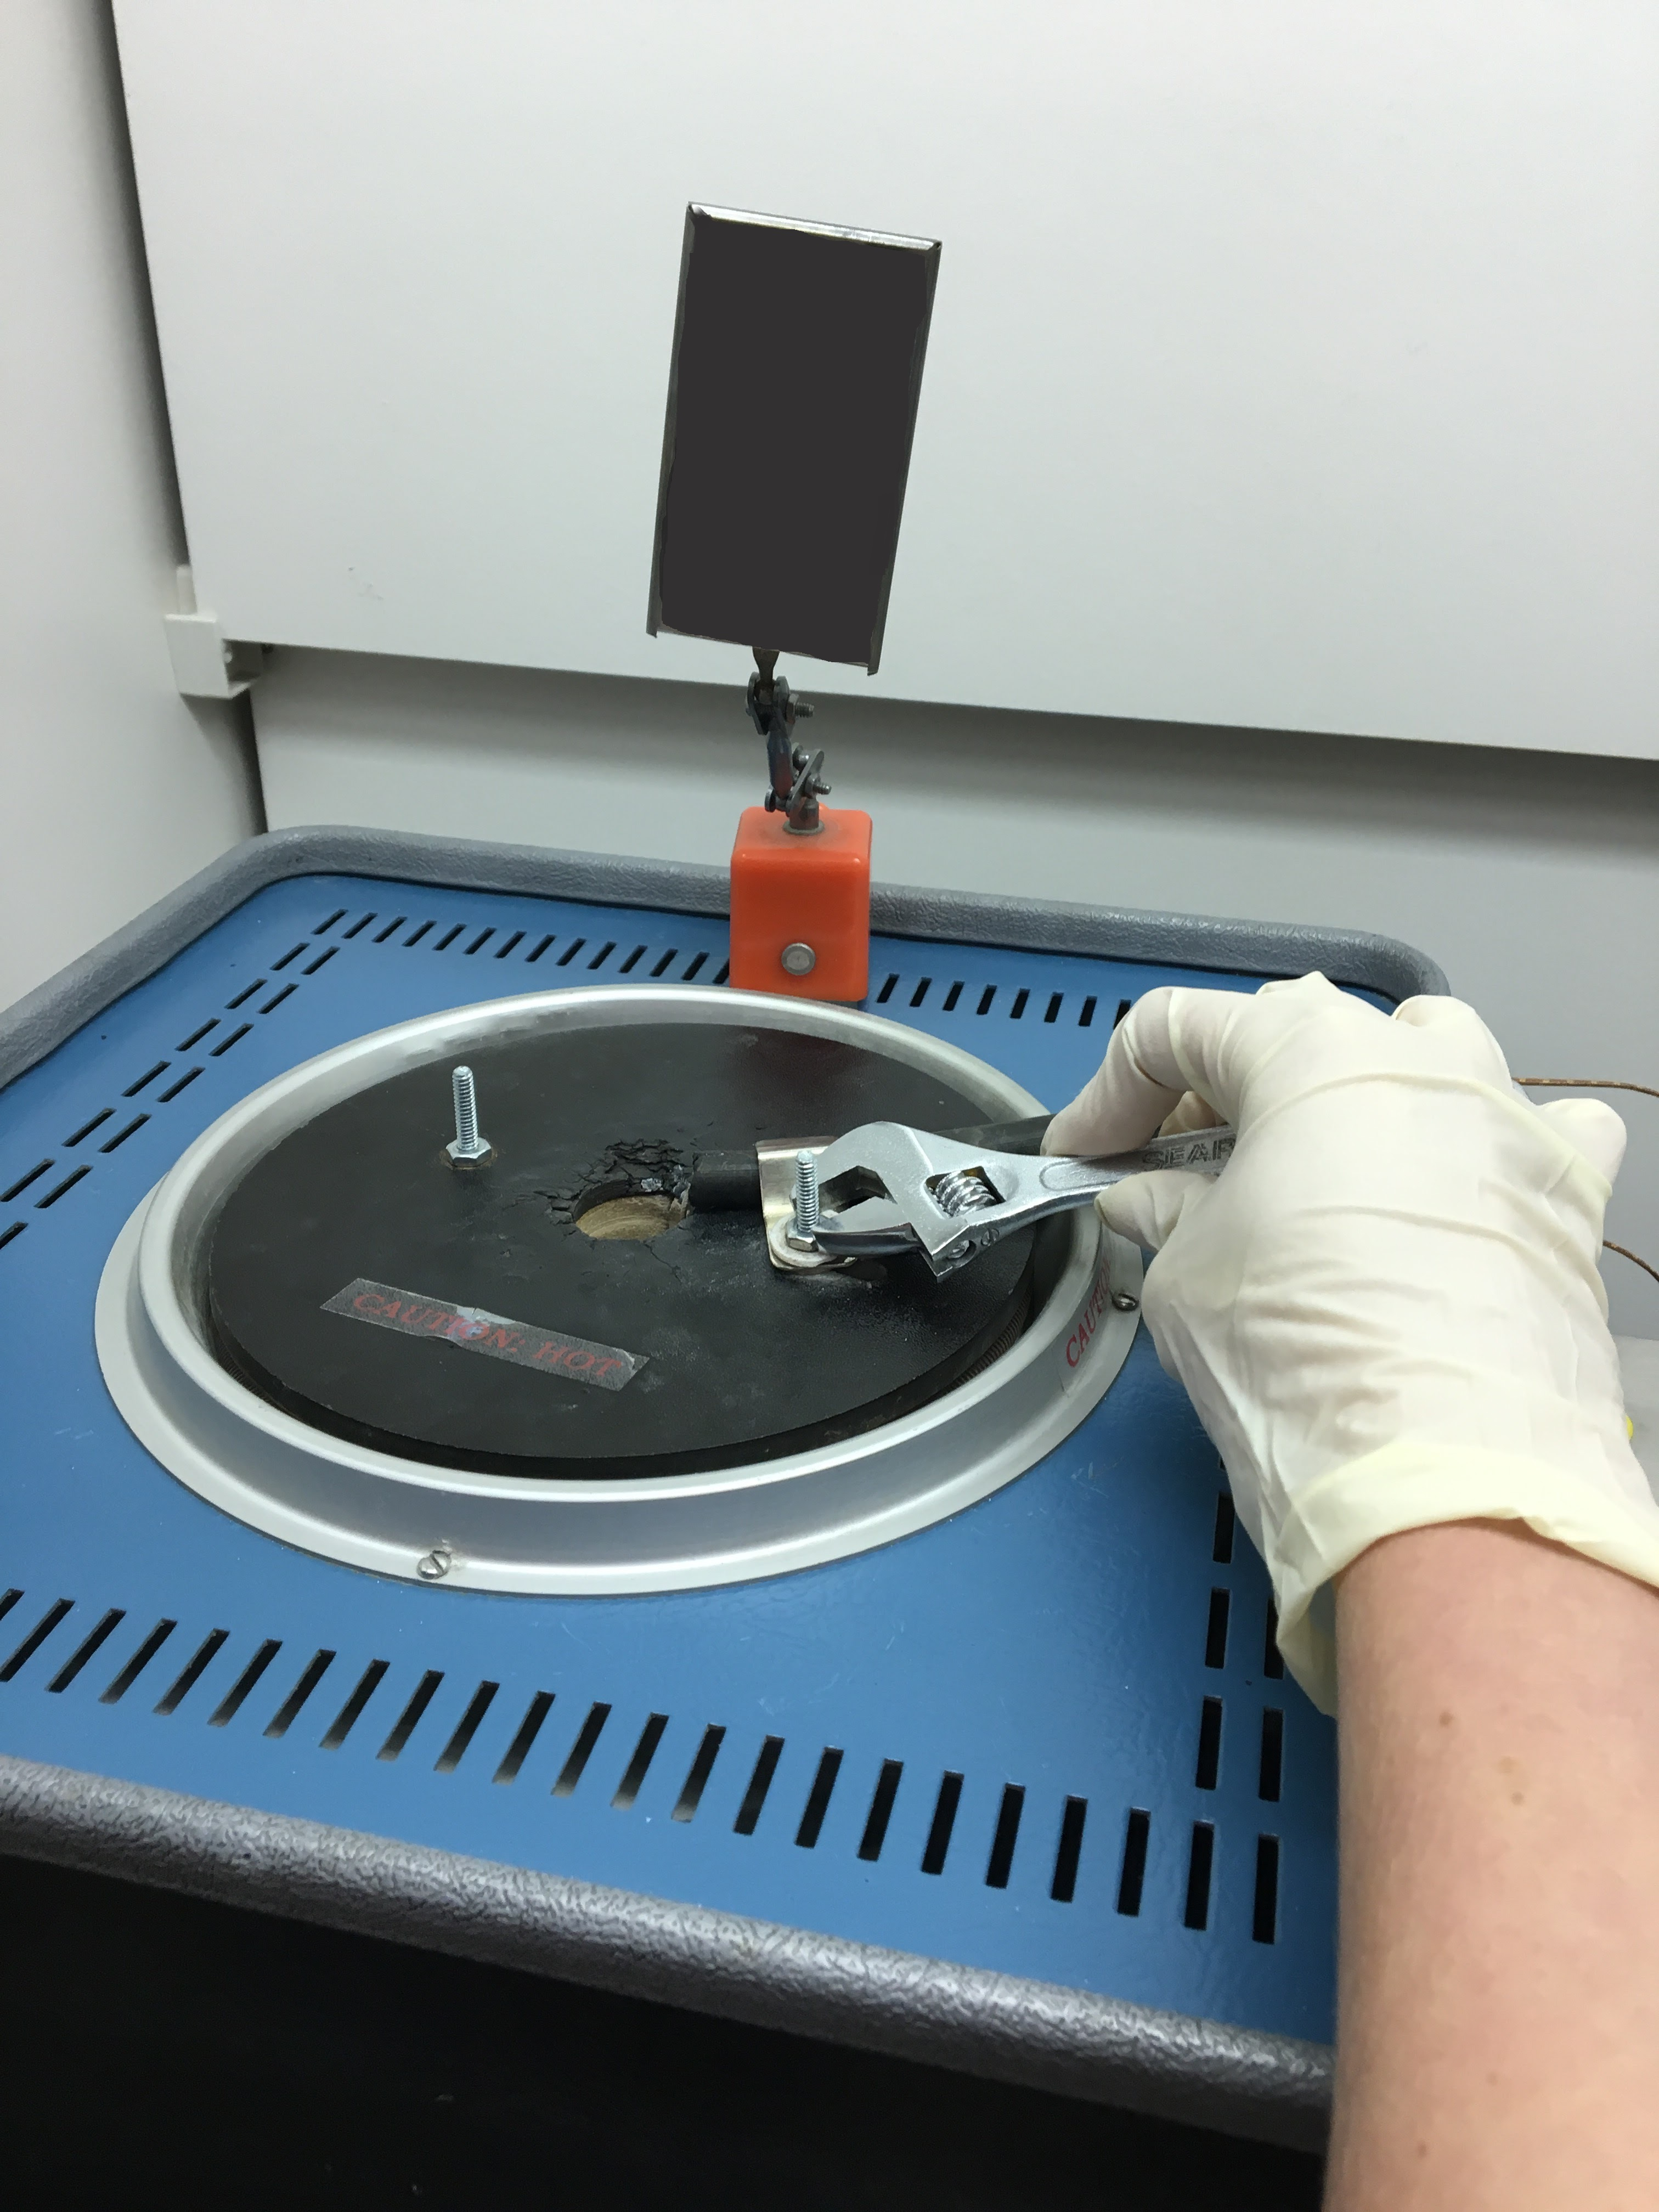
\includegraphics[width=.35\textwidth]{top_of_furnace_w_wrench.jpg}
\caption{Position thermocouple 4 with the rubber hose and tighten}
\label{fig:wrench_tight}
\end{figure}

        \item Connect the thermocouple connectors to join the  
            leads from the flask to the TADA, keeping the wires out of the way
            of the ARIA and tucked down to the side of the furnace
        \item Ensure the mirrors are set up correctly
        \item The final setup should resemble Figure \ref{fig:in_furnace}
        \end{itemize}
    
\begin{figure}[H]
\centering
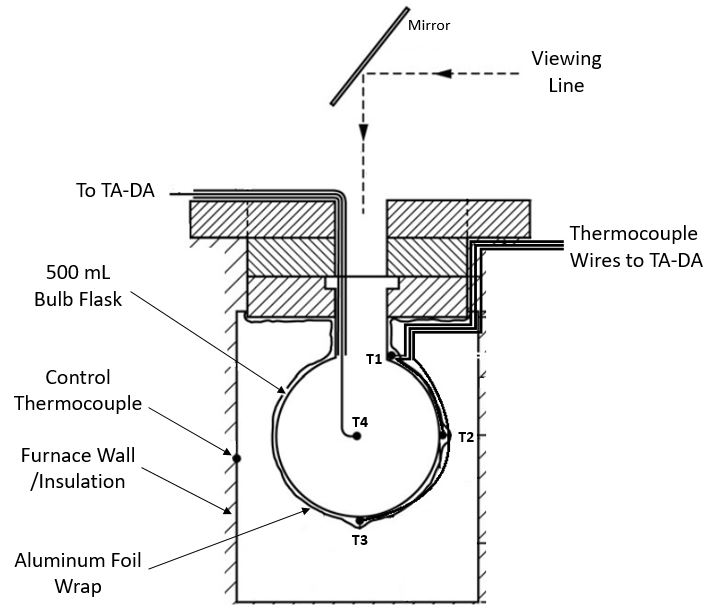
\includegraphics[width=.65\textwidth]{Furnace_diagram_mod.jpg}
\caption{Diagram of the furnace when assembled}
\label{fig:in_furnace}
\end{figure}

    \item Flask Cleaning \newline
        For consistent experimental results, flasks must be as clean as possible
        (See Figure \ref{fig:clean_dirty}). Dirty flasks can terminate radical 
        reactions and artificially raise the AIT. To ensure flasks are as clean 
        as possible before use, the following steps are required for flask 
        cleaning:
        \begin{itemize}
                \item Always begin by soaking the inside of the flask with soapy water 
            for 12 - 24 hours, regardless of how dirty it is
        \item While soaking, the flask should always be secured to a ring stand
        \item Wash out flask with soap and water, scrubbing the inside with 
            tube brushes
        \item For difficult stains, soak the flask inside with soapy water for 
            another 24 hours or longer if needed 
            \begin{itemize}
            \item During this process, scrub the inside and replace the 
                soapy water on a regular basis (generally every 12 - 24 hours)
            \end{itemize}
        
        \item Once all stains have been eradicated from the inside of the flask
            and the flask has been scrubbed in soapy water, rinse the inside and
            outside of the flask thoroughly
            \begin{itemize}
            \item Using hot water for rinsing is preferred but not required
            \item Rinse with tap water a minimum of 3 times, filling the flask
                with water, agitating the water for about 10 seconds, and then 
                dumping the water
            \item Repeat this process with distilled water available from the 
                smaller tap on the Northeast corner of the lab sink
            \end{itemize}
        
        \item If hard water spots or salt deposits appear on the inside of the 
            flask, rinse the inside of the flask with a small amount of vinegar
            to remove the deposits and repeat the rinse procedure above
        \item Once the flask has been cleaned and rinsed thoroughly, place the 
            clean flask on the drying rack over the sink
        \end{itemize}        
    \end{itemize}

\begin{figure}[H]
\centering
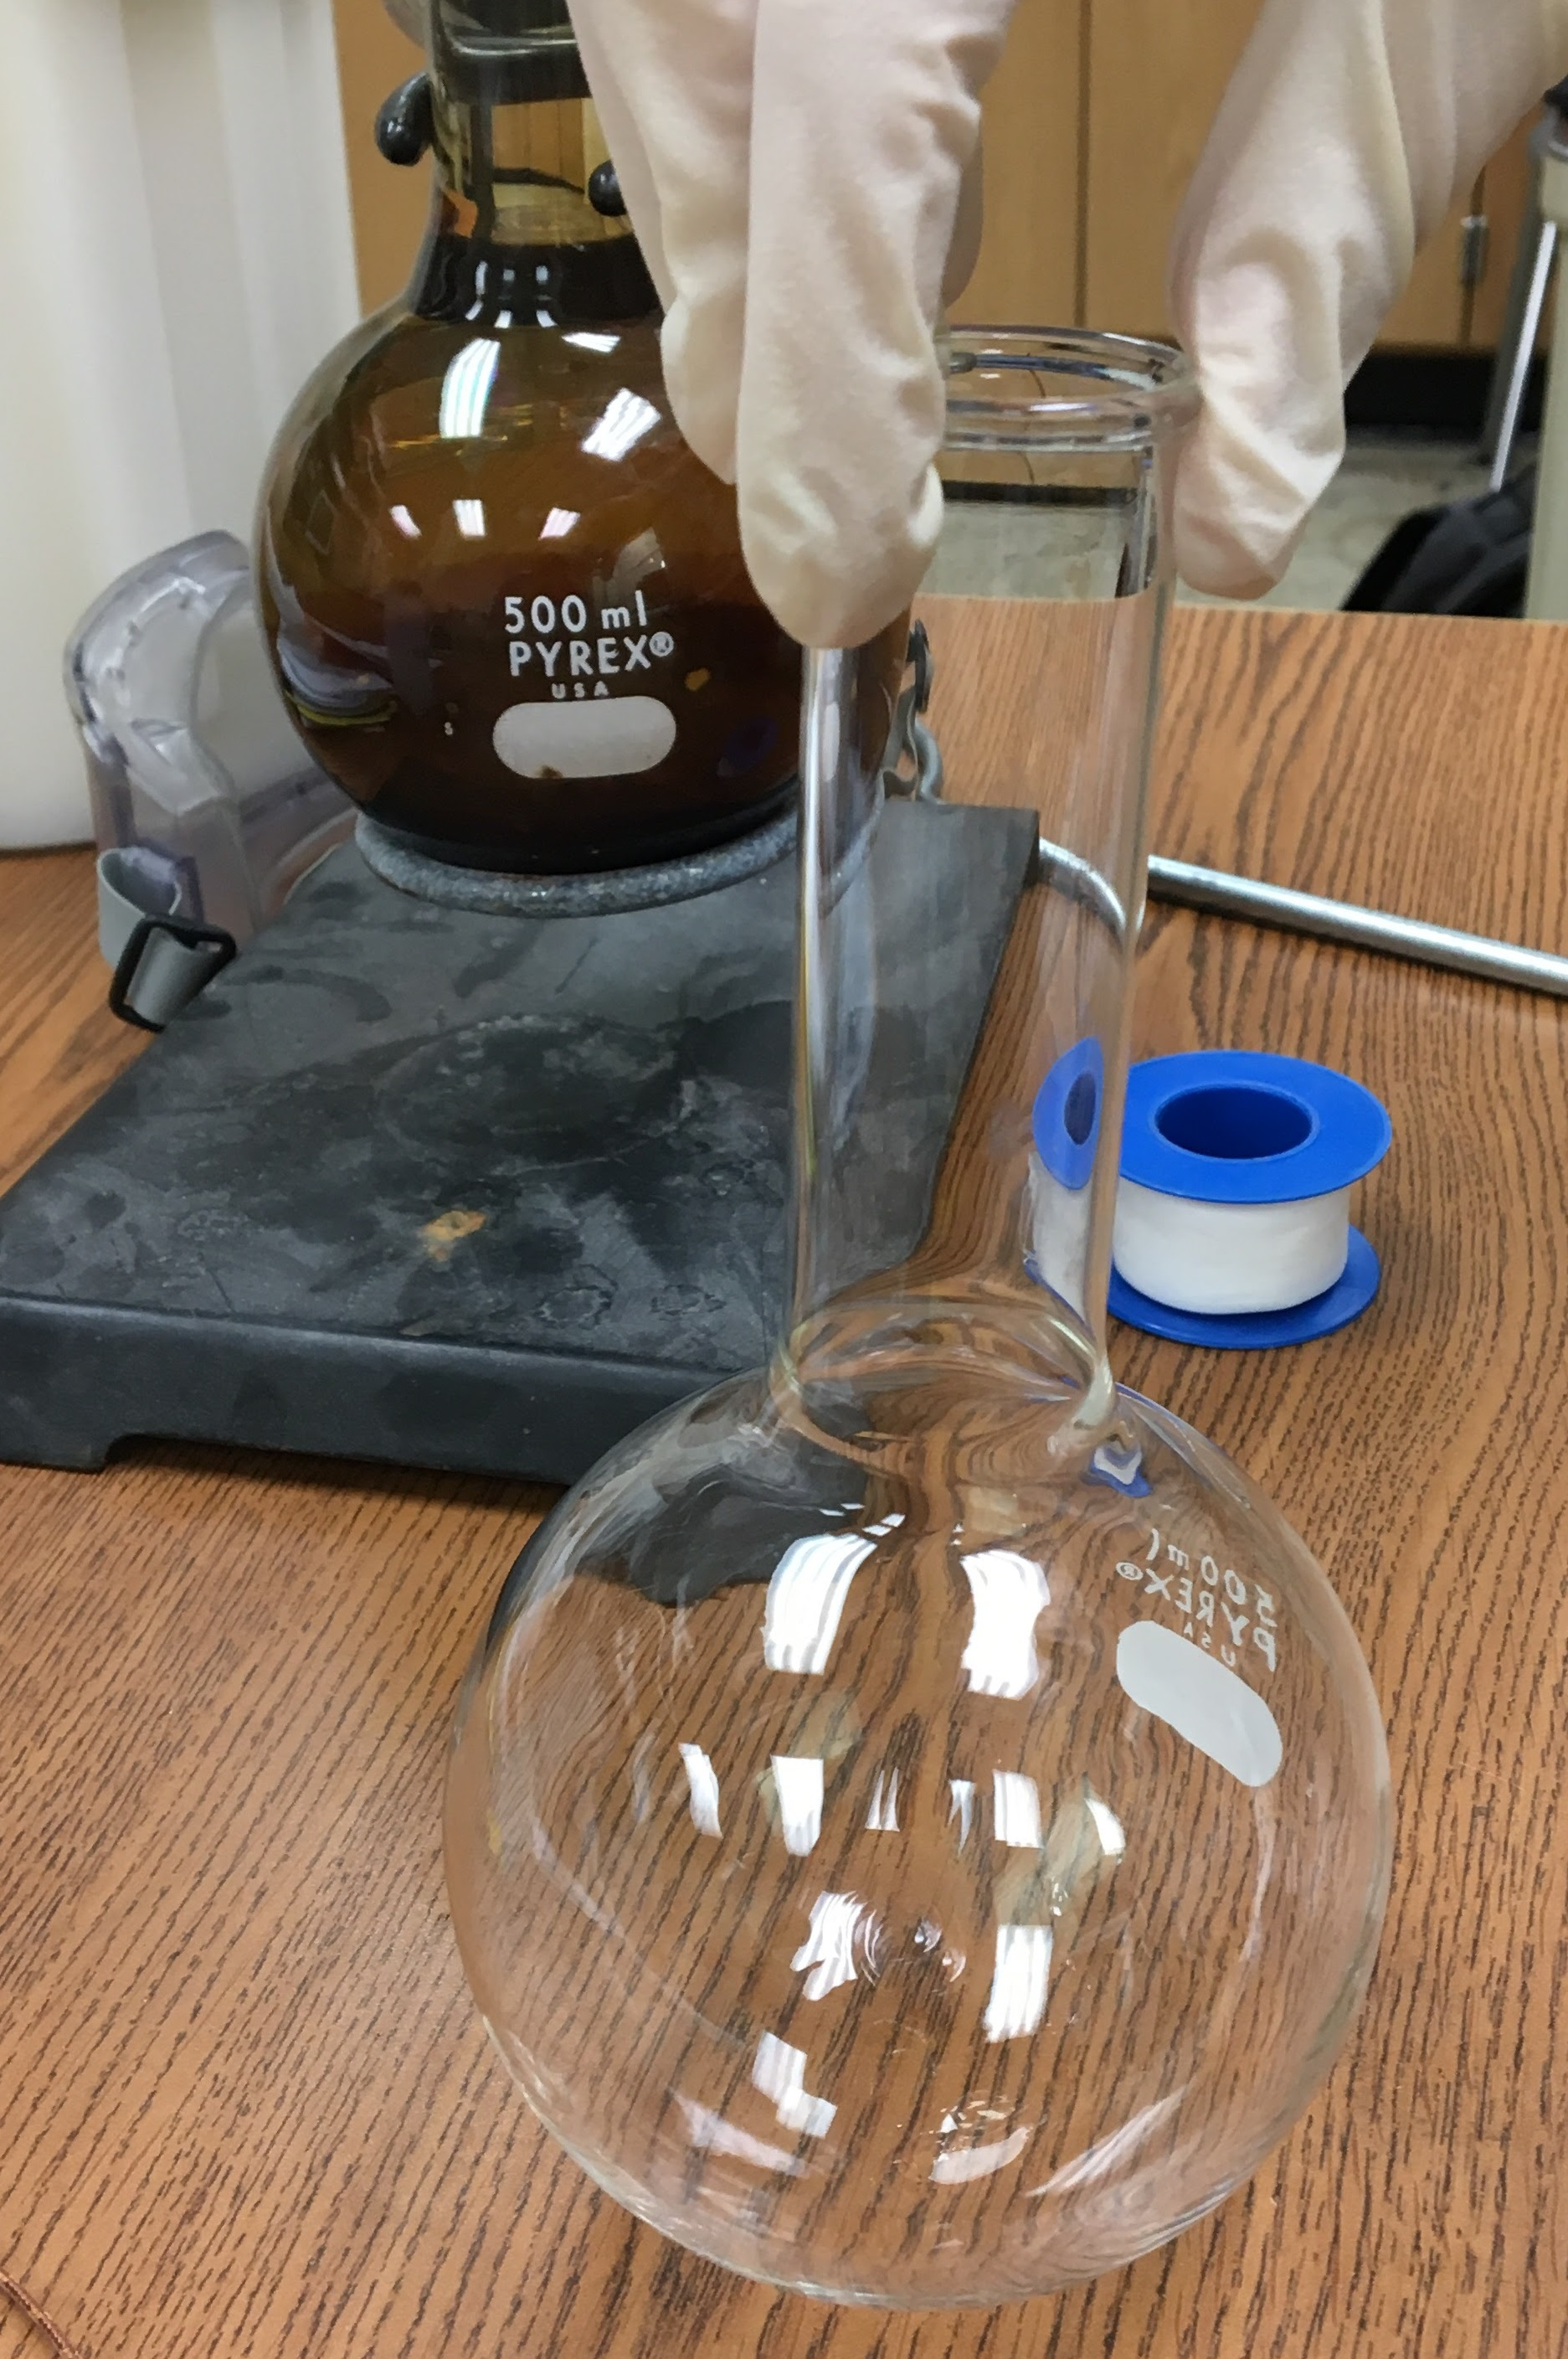
\includegraphics[width=.25\textwidth]{clean_dirty_flask.jpg}
\caption{A clean flask (dirty flask in the background)}
\label{fig:clean_dirty}
\end{figure}      

\end{document}
